\documentclass[12pt, ngerman]{article}

\usepackage[a4paper, inner=2.5cm, outer=2.5cm, top=2.5cm, bottom=2cm, bindingoffset=0cm]{geometry}

\title{\Large{\textbf{3D-Tracking-System auf Basis herkömmlicher Kameras}}}
\author{Alexander Minor}

% german shit
\usepackage[german]{babel}
% german quotes
\usepackage{csquotes}
\MakeOuterQuote{"}
% pictues and shit
\usepackage{graphicx}
\graphicspath{{assets/}}
% font carlito (calibri on crack)
\usepackage[sfdefault]{roboto}
% Used to wrap text around pictures
\usepackage{wrapfig}
% Used to compact list es
\usepackage{enumitem}
% Used to customize the page layout of your LaTeX documents
% \usepackage{fancyhdr}
% Blocksatz
\usepackage{ragged2e}
% Used to create an index
\usepackage{index}
% caption style
\usepackage[font=small]{caption}
\usepackage{subcaption}
\usepackage{caption}
\addto\captionsgerman{\renewcommand{\figurename}{Abb.}}
% configure spacing
\usepackage{setspace}
% make figures not go brr
\usepackage{float}
% Bibtex Literaturverzeichnis
\usepackage{cite}
% Math
\usepackage{amsmath}


\onehalfspacing
\setlength{\intextsep}{0pt}
\setlength{\parindent}{0cm}
\setlength{\parskip}{0.3cm}

% \renewcommand\cftchapafterpnum{\vskip10pt}
% \renewcommand\cftsecafterpnum{\vskip45pt}

\makeindex

%%%%%%%%%% Startseite
\begin{document}
% \begin{titlepage}
%   \begin{center}
%     \vspace*{3cm}

%     {\LARGE{3D-Tracking System auf Basis herkömmlicher Kameras}}

%     \vspace{0.5cm}
%     {\normalsize{Alexander Minor}}

%     \vspace{3.5cm}

%     \raggedright{\textbf{Schule:} Klaus-Groth-Schule Neumünster} \\
%     \vspace{0.2cm}
%     \raggedright{\textbf{Referenzfach:} Informatik/Mathematik} \\
%     \vspace{0.2cm}

%   \end{center}
% \end{titlepage}

%%%%%%%%%% Inhaltsverzeichnis
% \newpage

\tableofcontents

\newpage

\section{Einleitung}
Kameras sind die mit Abstand vielseitig nutzbaren Sensoren, denn einem Bild oder Video allein können viele Information über die Umgebung oder ein bestimmtes Objekt entnommen werden. Ohne weitere bekannte Parameter und Informationen können jedoch nicht mehr als zweidimensionale Projektionen der realen Welt akkurat erschaffen werden. In den letzten Jahren entwickelte sich für dieses Problem das sogenannte 3D-Tracking, bei dem mithilfe mehrerer statisch positionierten visuellen Sensoren die Position eines Objektes im dreidimensionalen Raum geschätzt werden kann. Diese revolutionären Systeme sind heute essenzieller Bestandteil vieler Gebiete, von der Filmproduktion bis zum autonomen Fahren. \par
\begin{wrapfigure}{r}{0.40\textwidth}
    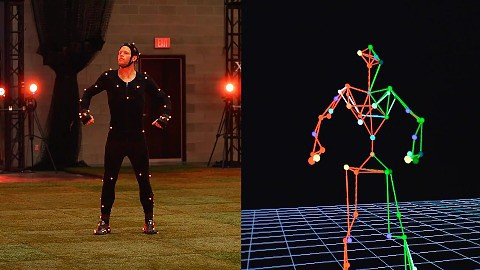
\includegraphics[width=\linewidth]{motion_capture_fifa.jpg}
    \caption{Motion Capture in der Filmproduktion}
    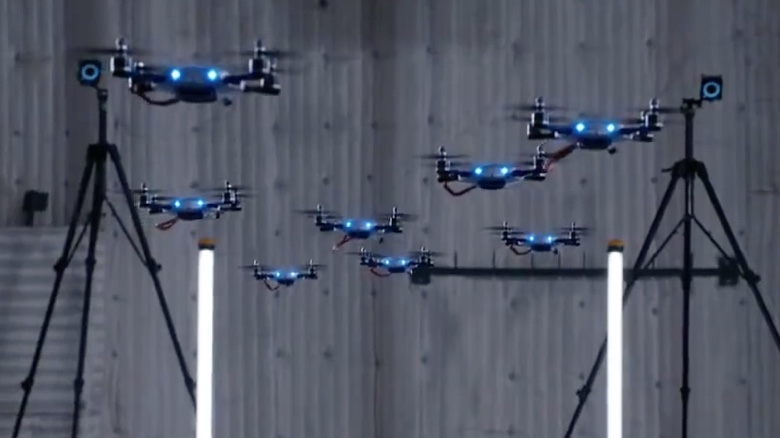
\includegraphics[width=\linewidth]{drones.jpg}
    \caption{Ein Schwarm von Drohnen kontroliert durch 3D-Tracking}
\end{wrapfigure}
In Filmen werden 3D-Tracking Systeme verwendet, um Bewegungen, Kämpfe und Szenen digital aufzuzeichnen und die gewonnenen Daten mit Hilfe computergenerierter Effekte zu den Szenen moderner Filme zu verwandeln, ohne die einzigartige Bewegungsart des Menschen zu verlieren (siehe Abbildung 1). 

Im Sport können Trajektorien eines Balles oder Bewegungen eines Spielers aufgezeichnet werden, um dem Training wichtige Informationen hinzuzufügen und auch in der Robotik ermöglicht das Tracking genau Steuerung und Korrektur von Drohnen oder Robotern. Nur durch die exakte Erfassung der Position können Fehler direkt oder im Voraus erkannt und korrigiert werden, die akkurate Positionierung und Bewegung des in Abbildung 2 zu sehenden Drohnen-Schwarm ist nur möglich, da eine zentrale Kontrolleinheit mithilfe der Daten aus einem 3D-Tracking-System die Bewegung der Drohnen hundertfach pro Sekunde anpasst. 
\subsection{Problematik}
\begin{wrapfigure}{r}{0.38\textwidth}
\centering
  \vspace{-40pt}
  {\setlength{\belowcaptionskip}{-20pt}
    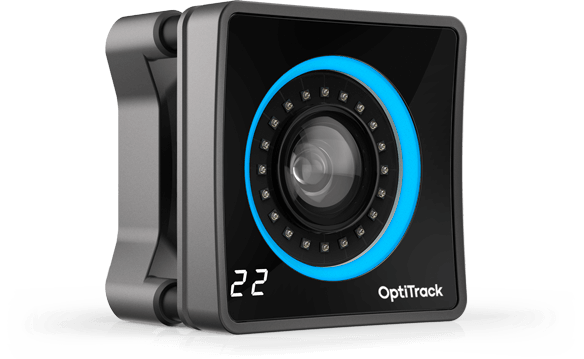
\includegraphics[angle=0,width=\linewidth]{4143.png}
    \caption{Optitrack UV-Tracking-Kamera}
  }
\end{wrapfigure}
Die Problematik, mit dem sich dieses Projekt befasst ist, dass es nur wenige Anbieter für solche Systeme gibt. Die Technik ist sehr teuer und nur gut finanzierte Projekte haben Zugriff auf diese revolutionären Systeme. Der bekannteste Anbieter Optitrack verlangt für die rechts gezeigt Kamera 4143\$, von denen für ein funktionierendes System mindestens 4 gebraucht werden. 

Das Ziel dieses Projektes ist es daher, ein Open-Source, günstiges und einfach zu integrierendes dreidimensionales Trackings-System zu entwickeln, damit Forscher, Entwickler und Interessierte auf der ganzen Welt, egal ob für Robotik, Filmproduktion oder der Messung von Bewegungen, 3D-Tracking als Basis für ihre Projekte verwenden können. \par
In dieser Projektarbeit wird die Theorie, der Entwicklungsprozess und die Ergebnisse meines 3D-Tracking Systems auf Basis herkömmlicher Webcams beschrieben und evaluiert.  
\newpage
\section{Vorgehen}
Bevor die tatsächliche Entwicklung der Software beginnen konnte, mussten zuerst die theoretische Funktionsweise und der grobe Aufbau des Systemes definiert werden.

\subsection{Theorie}
In einer Aufnahme einer herkömmlichen Kamera lässt sich die Position eines Objektes im zweidimensionalen Raum mithilfe von Object Tracking erfassen. Erweitert man diese Informationen mit den intrinsischen Werten der Kamera, also Brennweite, Verzerrung und Skalierung, in den dreidimensionalen Raum, fehlen einem die nötigen Informationen, um die Tiefe, also die Entfernung zur Kamera, zu berechnen.  

\begin{wrapfigure}{r}{0.38\textwidth}
\centering
  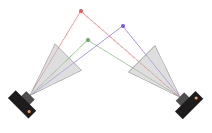
\includegraphics[angle=0,width=\linewidth]{triangulation.png}
  \caption{Epipolargeometrie zweier Perspektiven}
\end{wrapfigure}
Es bleibt also eine Gerade, auf der sich das Objekt befinden könnte. Wenn man nun eine zweite Kamera hinzufügt, erhält man eine weitere Gerade, auf der sich das Objekt befinden könnte. Liegen die Kameras an unterschiedlichen Orten, lässt sich die akkurate Position des zu trackenden Objektes durch den Schnittpunkt der beiden Geraden berechnen (siehe Abbildung 4). Wenn man jegliche Messfehler vernachlässigt, und die exakte Position der Kameras bekannt ist, würden zwei Kameras schon ausreichen, um die nötigen Daten zur Berechnung zu liefern.  

In der Realität gibt es aber einige Aspekte, die die Genauigkeit und Funktionalität des Systems negativ beeinflussen: 
\begin{itemize}
  \item Da ein Bild einer Kamera eine begrenzte Auflösung hat, kann eine Kante eines Objektes nur die Hälfte eines Pixels ausfüllen. Durch das „Auf- oder Abrunden“ dieser Bildinformationen entsteht ein Messfehler, der mit zunehmender Distanz größer wird. 
  \item Da die verwendeten Kameras  nur selten Informationen zu den intrinsischen Daten mitliefern, lassen sich diese nur mithilfe einer Kalibrierungssequenz ermessen. In der werden mehrere aufgenommen verzerrte Bilder so angepasst, dass sie den tatsächlichen Eigenschaften eines bekannten Objektes nahekommen, in der Praxis ist dies meist ein Schachbrett. In der resultierenden Projektion der Aufnahme im dreidimensionalen Raum können durch Messfehler Verzerrungen oder Verschiebungen entstehen. 
  \item Der mit Abstand stärkste Einfluss auf mögliche Fehler ist die durch eine Kalibrierungssequenz geschätzte Position der Kameras. Sowohl Rotation und Transposition zur Uhrkamera müssen perfekt sein, damit tatsächlich ein Schnittpunkt entsteht. 
\end{itemize}

Es wird also ersichtlich, dass ein perfekter Systemaufbau aufgrund der vielen Variablen nicht realistisch ist, und die Position des getrackten Objektes angenähert werden muss. Um diese möglichst nahe an die tatsächlichen Werte zu bringen, gibt es folgende Möglichkeiten: 
\begin{itemize}
  \item Eine größere und besser verteilte Anzahl an Kameras. Der kleinste Fehler für die Annäherung eines möglichen Schnittpunktes verschiedener Geraden entsteht dann, wenn diese orthogonal zueinander verlaufen. Es ist also vorteilhaft die Kameras möglichst effektiv im Raum zu positionieren. Auch die Anzahl verringert den Fehler, da einerseits mehr Daten entstehen und anderseits beim Ausfall oder starkem Messfehler nicht gleich das ganze System zusammenbricht. 
  \item Ein Algorithmus zum Erkennen von starken Messfehlern und guter Annäherung eines möglichen Schnittpunktes. 
\end{itemize}

\newpage
\subsection{Technische Voraussetzungen}
Bevor es an die tatsächliche Entwicklung gehen kann, müssen einige Spezifikationen, Voraussetzungen und zu verwendende Systeme definiert werden, damit das grobe Konzept auch tatsächlich umsetzbar ist. Dazu gehört die verwendete Hardware in Form von Kameras und Software in der Form von Programmiersprache, Bibliotheken und Programmen zur Entwicklung und Visualisierung. 

\subsubsection{Python}
Da das Projekt komplex ist, ist eine „high-level“ Programmiersprache zu präferieren, wodurch komplexere Aufgaben mit weniger Befehlen gelöst werden können. In diesem Bereich bietet sich Python besonders an, da diese einerseits großen Support in Form von zahlreichen Libraries und einer aktiven Community besitzt und ich andererseits bereits viel Erfahrung in diesem Bereich hatte. 

\subsubsection{ROS}
Das zu entwickelnde System sollte besonders variabel, erweiterbar und vielseitig nutzbar sein, es ist daher sinnvoll den Code modular aufzubauen, sodass bestimmte Teile ausgetauscht, verbessert oder erweitert werden können, ohne die Funktionalität des ganzen Systems zu hindern.  

Um eine solche Modularität schaffen zu können, werden bestimmte Vereinbarungen und Vorgaben gebraucht, wie zwischen Teilen kommuniziert werden soll, wie diese voneinander abhängig sind und wie die generelle Struktur des Systems aussieht.  

So wäre es beispielsweise sinnvoll, das Auslesen, Verarbeiten und Vergleichen der Kamerabilder voneinander zu separieren, sodass einerseits eine gewisse Unabhängigkeit entsteht und andererseits so von Multithreading Nutzen gemacht werden kann, der Aufteilung der Rechenlast auf mehrere CPU-Kerne.  

Auch wenn zahlreiche Lösungen für das Aufteilen eines Python-Programmes in verschiedene Threads (Unterprogramme) bereits nativ möglich ist, wäre die Integration in komplexere Systeme äußerst mühselig, da vor allem die Kommunikation in Form von geteilten Variablen eher primitiv und zeitlich aufwändig wäre. Es musste also ein System her, dass die Kommunikation und Separierung der Programme vereinfachen würde und idealerweise bereits vorgefertigte System für kleinere Aspekte des Projektes hätte, sodass bei der Entwicklung auf bereits getesteten Code zurückgegriffen werden konnte. 

\begin{wrapfigure}{r}{0.38\textwidth}
\centering
  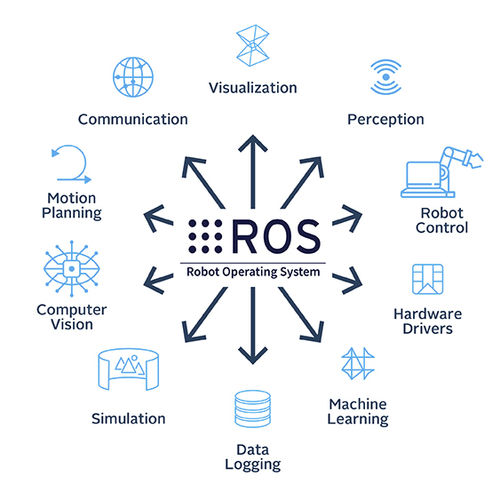
\includegraphics[angle=0,width=\linewidth]{ROS_diagram.jpg}
  \caption{Anwendungen von ROS}
\end{wrapfigure}
Alle diese Voraussetzungen erfüllte das Open-Source System „ROS“ (Robotic Operation System), ein seit 2007 entwickelte Framework für Roboter, welches in zahlreichen persönlichen und industriellen Systemen verwendet wird. ROS, oder im Falle dieses Projektes die zweite Version ROS2, ist weniger eine Library für eine bestimmte Programmiersprache, sondern wie im Namen schon enthalten, ein „Operating System“, also eine Vielzahl an Libraries, Tools und Algorithmen für die Entwicklung von Robotern, die tiefer im System integriert sind. Der Code selbst wird dann in Python geschrieben, und kann mithilfe einer Library (rclpy) mit ROS kommunizieren. 

ROS ermöglicht es nun, sogenannte „Nodes“ zu erstellen, diese sind unabhängige Module, die in ihrer eigenen Python oder C++ Datei erstellt werden können. So gibt es beispielsweise für jede Kamera eine Node, die sich nur um das Auslesen der Bilder kümmert, eine weitere zum Erkennen verschiedener Objekte und eine andere zum Vergleichen dieser Daten mit anderen Kameras.  

Allein können diese Module allerdings nichts erreichen, da sie von Informationen untereinander abhängig sind. Auch hier bietet ROS zwei zentrale Tools zur Kommunikation zwischen Nodes:  

\begin{itemize}
  \item Das Publisher-Subscriber Modell, in dem die Kommunikation stets nur in eine Richtung läuft. Wie in Abbildung 6 zu sehen, veröffentlicht der Publisher eine Nachricht mit bestimmten Parametern (Message) auf einem Topic, auf dem mehrere Subscriber "zuhören" können. 
  \begin{figure}[h]
    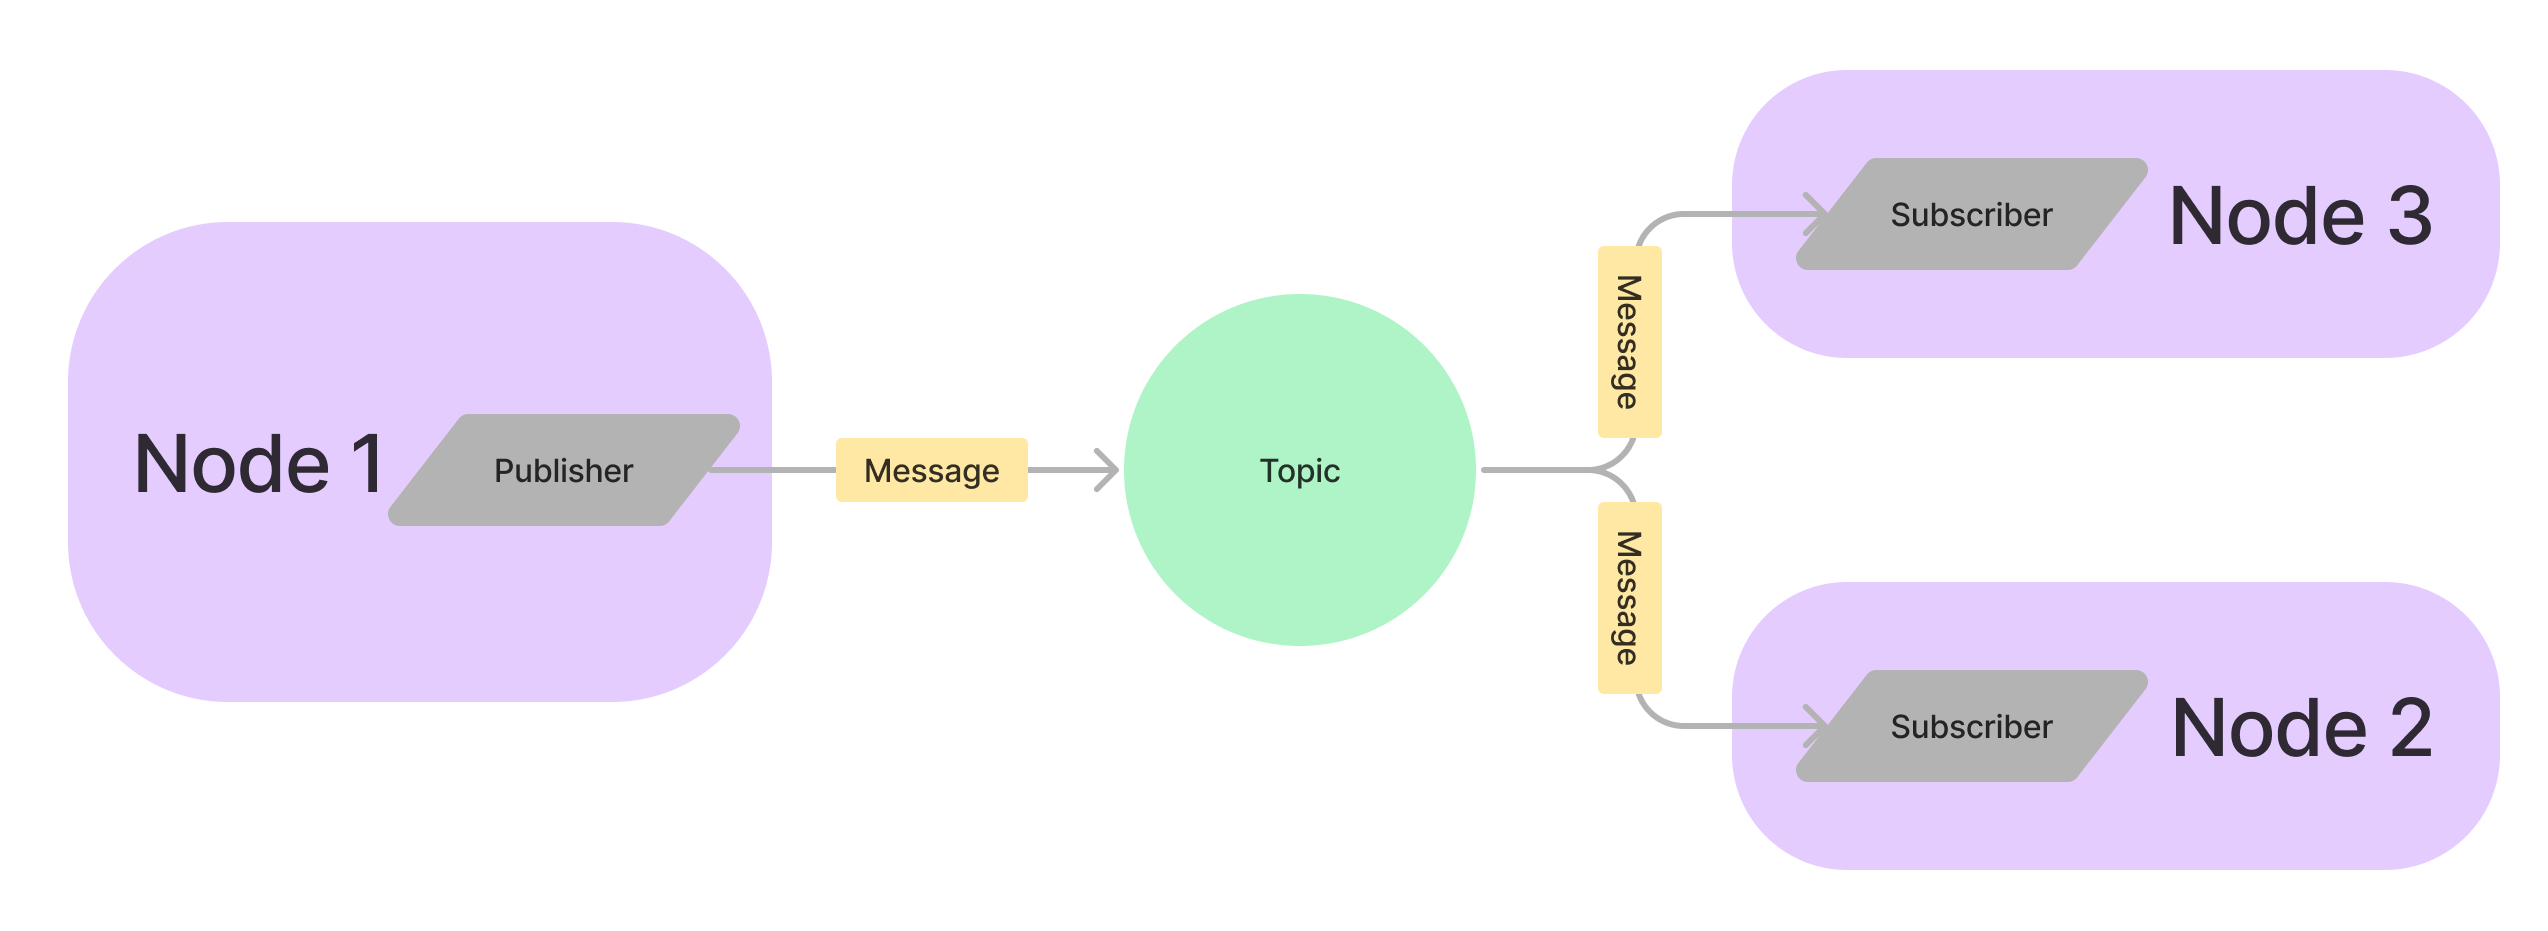
\includegraphics[angle=0,width=\linewidth]{Publisher.png}
    \caption{Publisher-Subscriber-Modell}
  \end{figure}
  \item Das Service-Modell, in dem die Kommunikation wie bei einem TCP-Handshake verläuft, also vom Client eine Anfrage zum Server gesendet wird und bei erfolgreicher interpretation eine Antwort zurück kommt. 
  \begin{figure}[h]
    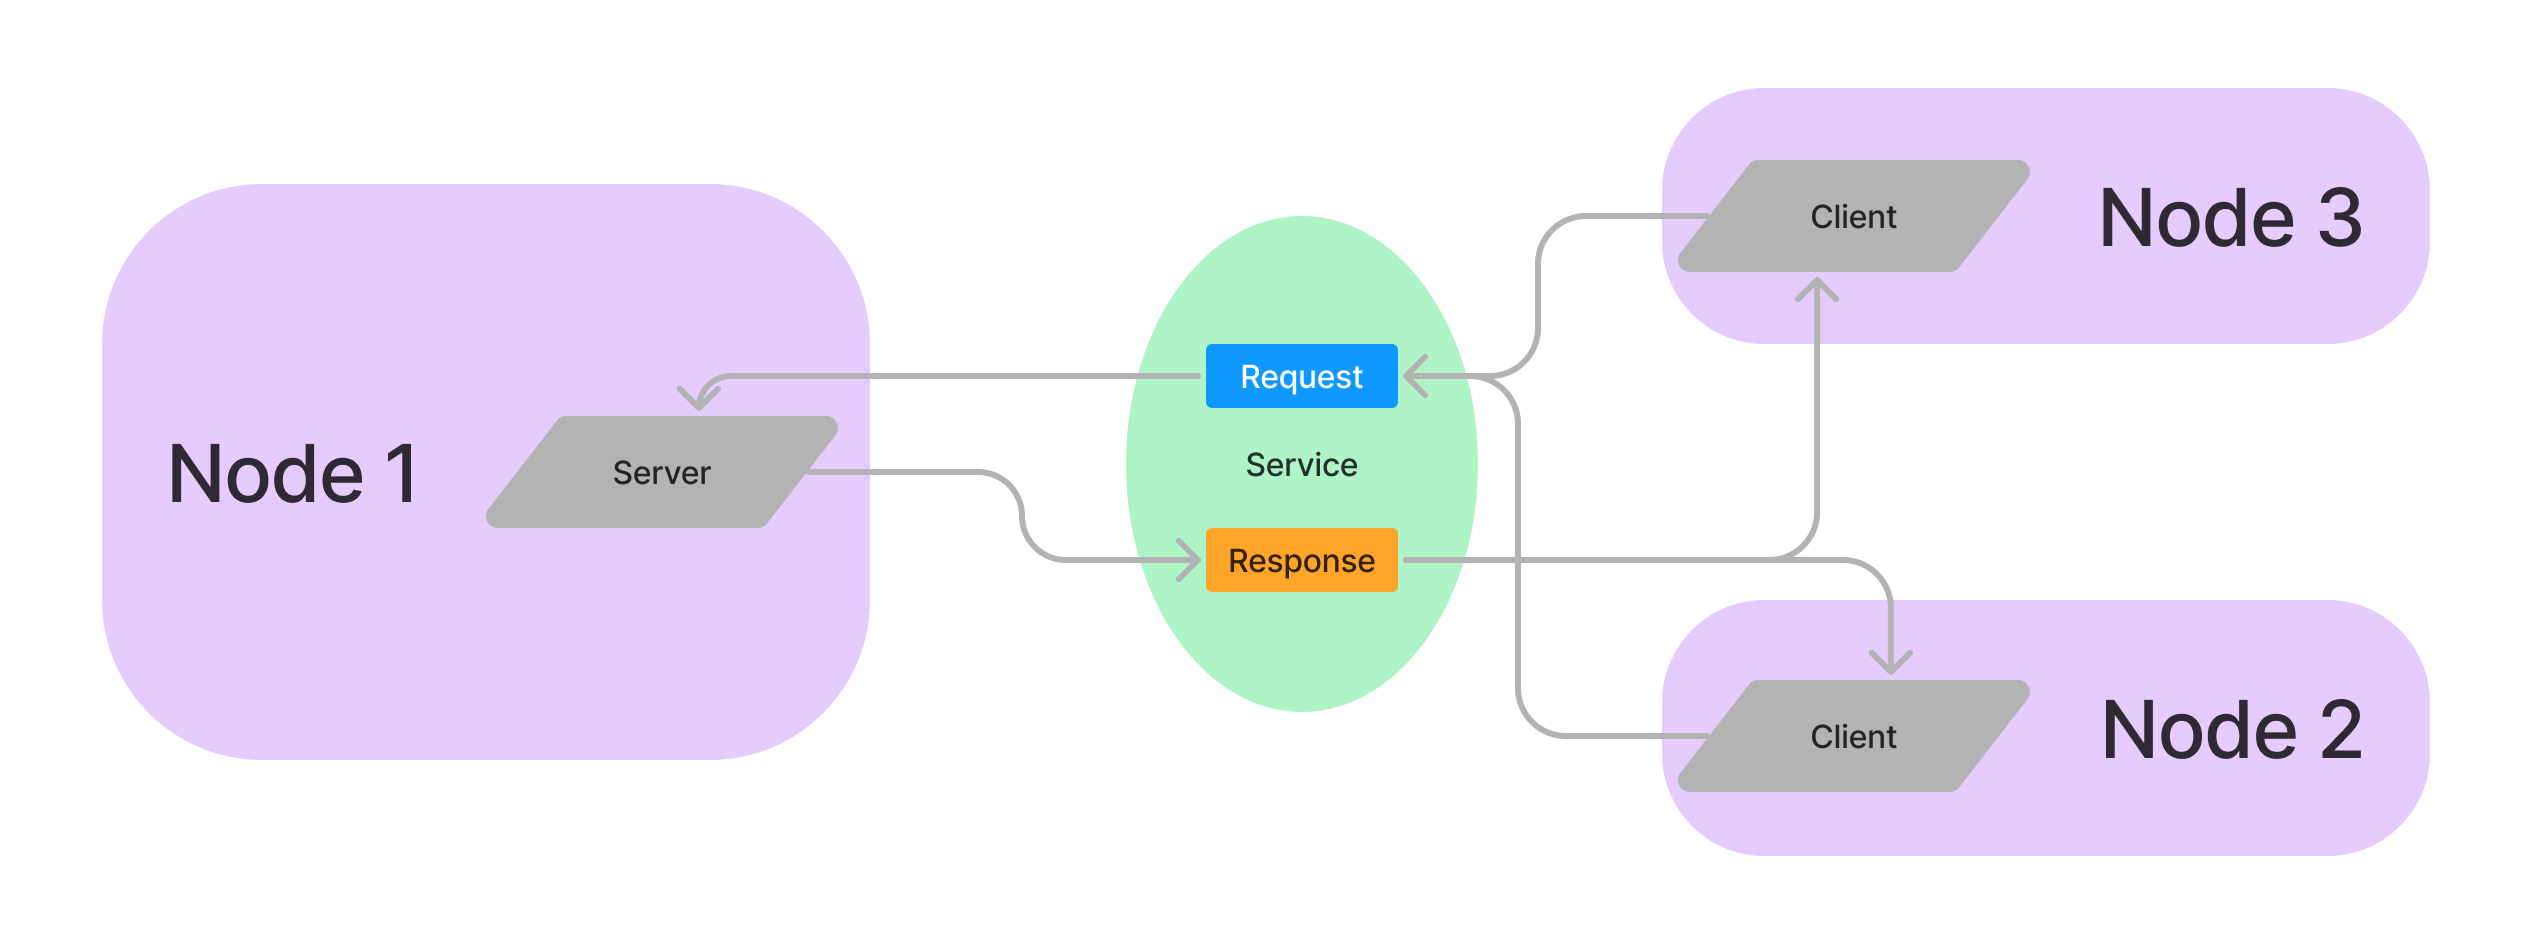
\includegraphics[angle=0,width=\linewidth]{Server.png}
    \caption{Server-Client-Modell}
  \end{figure}
\end{itemize}

Da alle Kommunikation meist einseitig sind und Geschwindigkeit eine wichtige Rolle spielt, wird im 3D-Tracking-System stets über das Publisher-Subscriber-Modell kommuniziert.

Ein weiterer Kernaspekt, weshalb ROS ein essenzieller Part dieser Entwicklung ist, hat mit der Etablierung der Technik zu tun. Da jede Art von Kommunikation durch sogenannte „Messages“ beschrieben wird, also welche Daten genau übertragen werden, gibt es viele Programme, die diese „verstehen“ können. Bilder, Vektoren, Kamera-Matrizen oder simple Punkte, werden daher immer auf dieselbe Weise versendet. So gibt es gute Möglichkeiten zur Visualisierung und Simulation der Daten, sowie zahlreiche andere Apps, die die Entwicklung durch ROS erleichtern. 
\subsubsection{Opencv}
Eine weitere Library, die in diesem Projekt eine große Rolle spielt, ist OpenCV, bzw. die Python Implementation. Dies ist eine freie Programmbibliothek mit Algorithmen für die Bildverarbeitung und Computer Vision. Durch sie wird sowohl das Auslesen der Kameradaten, als auch die Kalibrierung zur Berechnung der intrinsischen Parameter möglich.
\subsection{Vorgehensweise und Wandel}
Um die Flexibilität und Zuverlässigkeit des Systems sicherzustellen, wurde in der Entwicklung jedes Modul ausgiebig getestet, sowohl separat als auch im System integriert. Das Vorgehen in der Programmierung war also stets mit dem Testen des Systems verbunden, weshalb jedes Modul kontinuierlich im Laufe des Projektes verbessert wurde, sobald Fehler entdeckt wurden oder neu Funktionalität nötig war. 

\section{Systemaufbau}
Jede Ausführung des Tracking-Systems startet mit dem sogenannten "Manager", dies ist ein Programm, welches nach angeschlossenen Kameras sucht und alle nötigen Nodes zum Tracking konfiguriert und startet. Ein laufendes System kann in etwa so aussehen:
\begin{figure}[h]
  \centering
  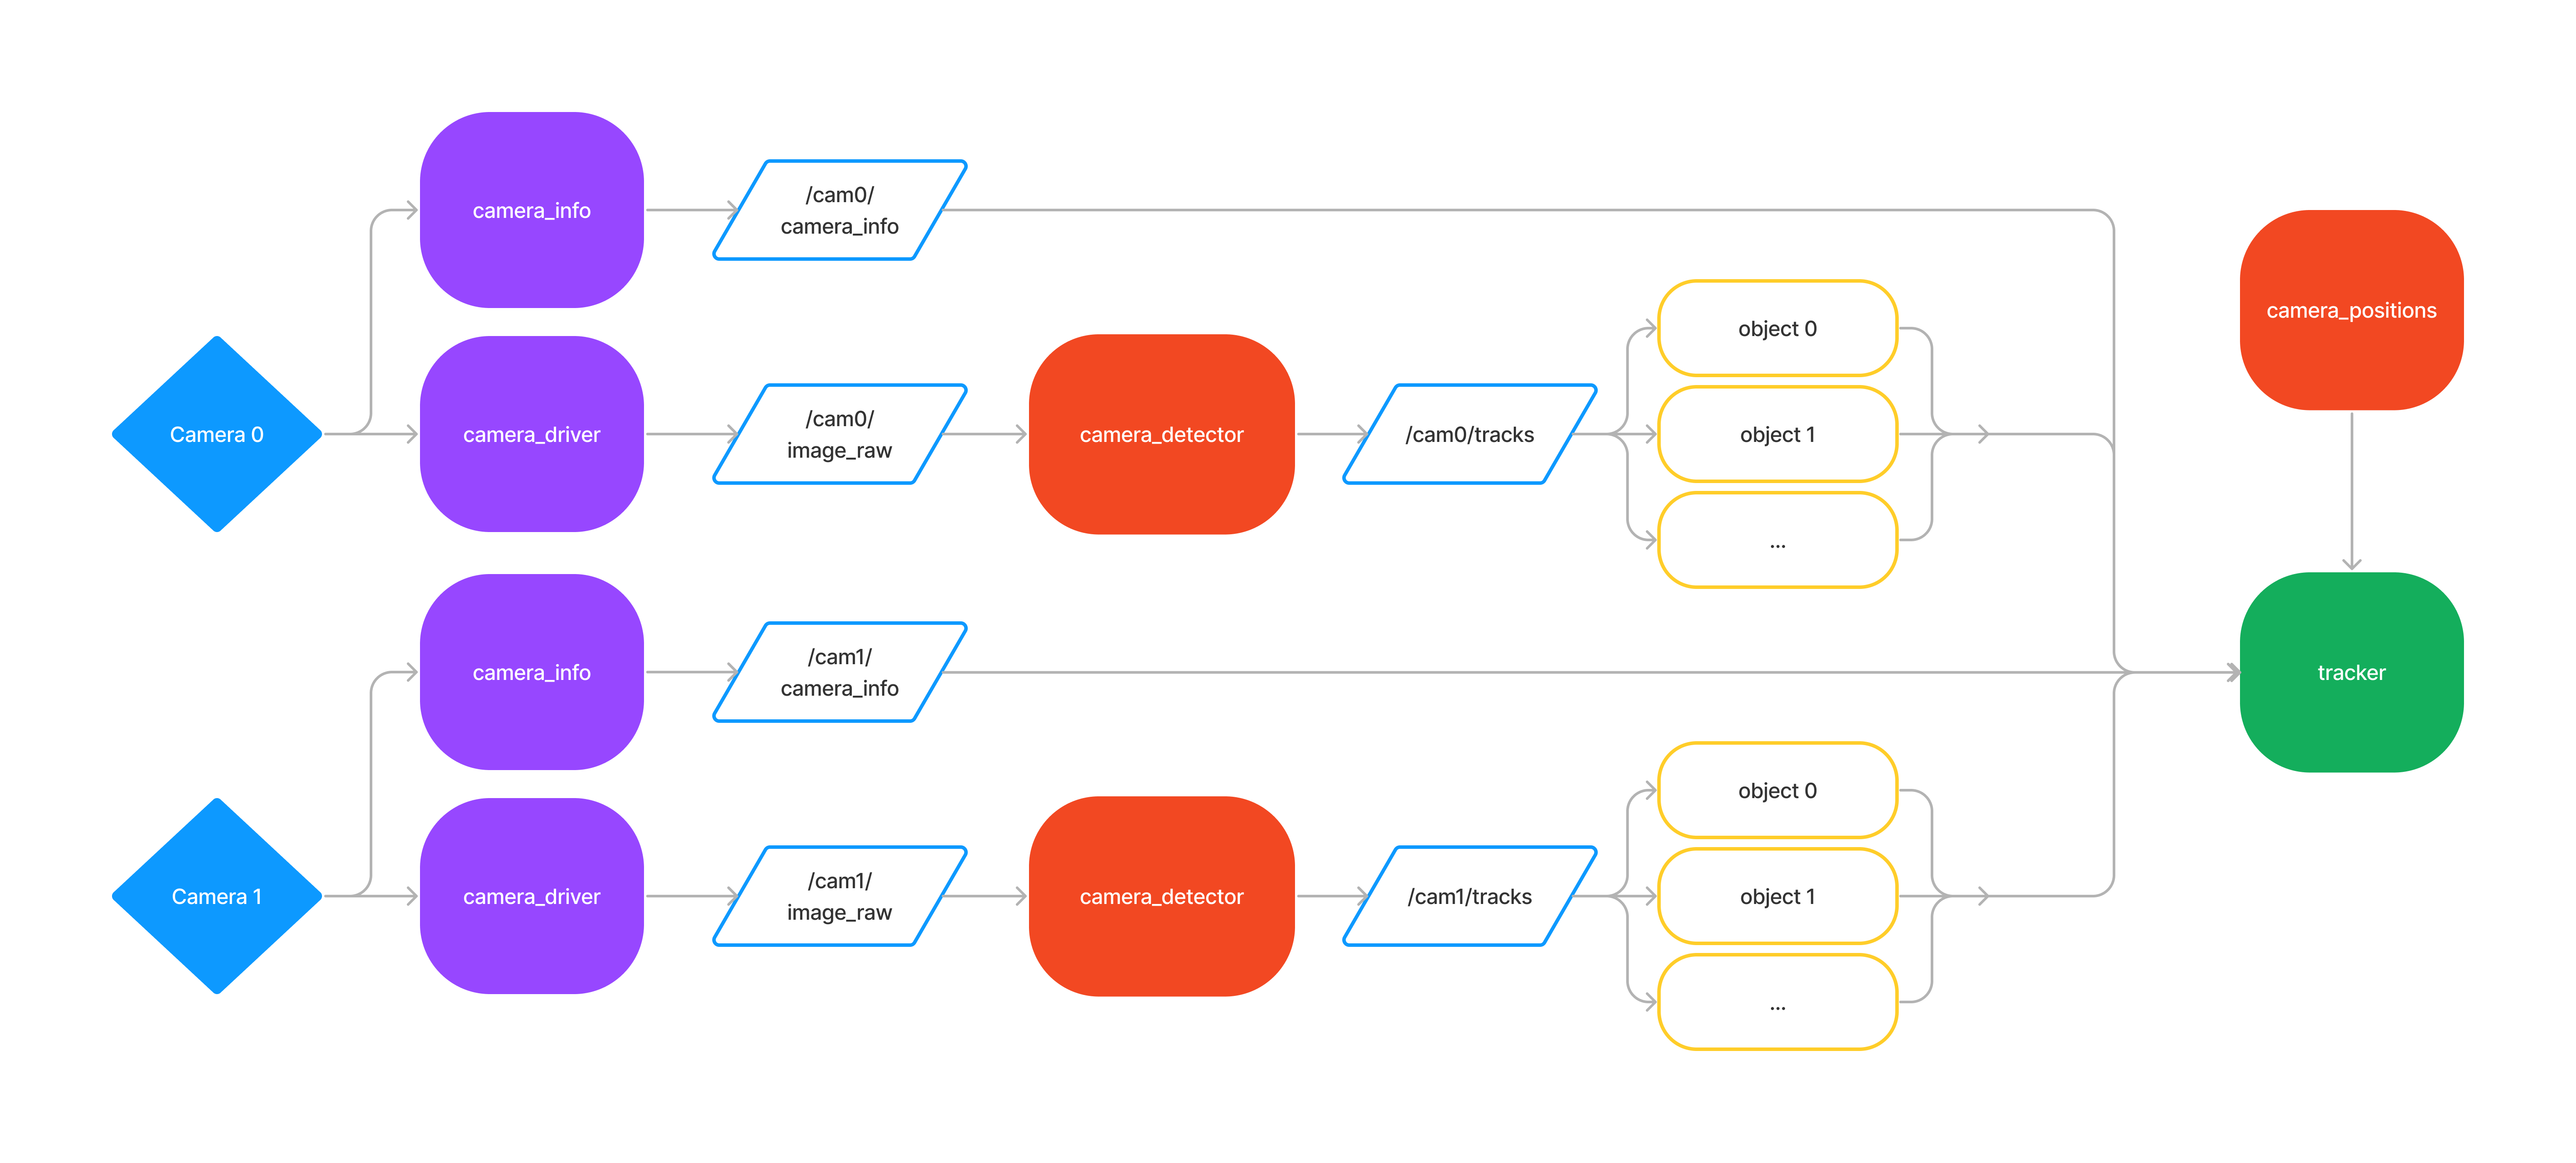
\includegraphics[angle=0,width=\linewidth]{anytrack-basic-tracking.png}
  \caption{Nodes, Topics und Messages eines laufenen Systemes mit 2 Kameras}
\end{figure}

Die Funktionalität und Aufgabe der einzelnen Module  wird im Folgenden erklärt:
\subsection{Driver}
Ursprünglich war das Auslesen und Verarbeiten der Bilder in einem Modul kombiniert, in dem eine kontinuierliche Schleife die Daten ausliest, verarbeitet und nach zu trackenden Objekten scannt. Im späteren Verlauf der Entwicklung zeigte sich jedoch, dass es nur durch die Separierung möglich ist, eine Simulationsumgebung möglichst direkt in das System zu integrieren. Dies ist nötig gewesen, da die Entwicklung des Kalibrierung-Prozesses zur Schätzung der Kamera Posen synthetische Daten gebraucht hat, um ein stabiles und stets identisches System zum Testen zu haben. 

Wenn die Bilder nicht von der Simulationssoftware gegeben werden, gibt der "camera\_driver" (siehe Abbildung 8) das Bild und den exakten Zeitpunkt der Aufnahme im ROS Netzwerk frei. Letzteres ist vor allem im später beschriebenen Kalibrierungsprozess wichtige, da ein zu großer zeitlicher Unterschied eine Fehlerquelle seien könnte.

\subsection{2D-Tracking}
Bevor die Position eines Objektes im dreidimensionalen Raum berechnet werden kann, müssen zunächst die zweidimensionalen Koordinaten des Objektes im Bild der Kamera errechnet werden, wofür das "camera\_detector" Modul zuständig ist. Als Tracking-Objekt dienen kleine hellgrüne Kugeln, da sie von allen Seiten gleich aussehen und gut vom Hintergrund zu unterscheiden sind. Diese Tracking-Objekte werden in fortan als "Marker" bezeichnet.  

Üblicherweise wird für solche Zwecke Object-Tracking verwendet, bei dem die bestimmten visuellen Eigenschaften eines Markers gespeichert und im nächsten Frame danach gesucht wird. Ein solches Objekt kann ein Auto, ein Mensch oder in diesem Fall eine Kugel sein.  

Auch wenn Object-Tracking mit Librarys wie OpenCV erstaunlich leicht zu integrieren ist, gibt es in diesem Fall eine simplere und schnellere Methode: Das Tracking von bestimmten Farb-Konturen, die nach dem Anwenden einer bestimmten „Maske“ übrigbleiben. 

Die Problematik bei dieser Technik liegt in der Unterscheidung des Objektes zum Hintergrund. In professionellen, aber sehr viel teuren Systemen, wird auf Infrarot-Kameras und besonders reflektierende kleine Kugeln gesetzt. Dieselbe Technik lässt sich aber auch auf herkömmlichen Webcams anwenden, wenn die Kugeln in einer besonders starken und im Hintergrund nicht vorhandenen Farbe sind. 

\vspace{10pt}
\begin{figure}[H]
  \begin{wrapfigure}{r}{0.4\textwidth}
    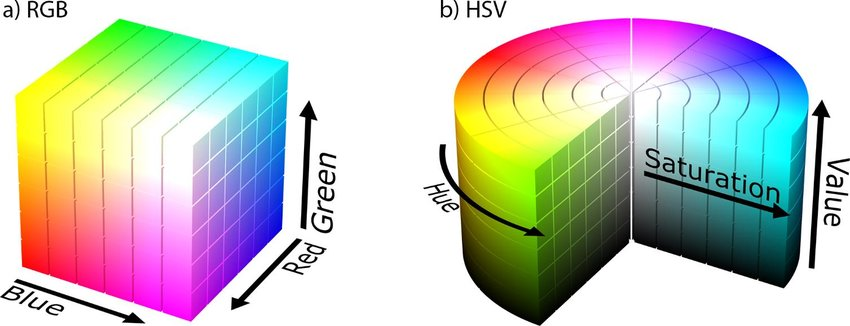
\includegraphics[angle=0,width=\linewidth]{rgb-hsv.png}
    \caption{RGB und HSV Farbformat}
    \label{Abb: HSV}
    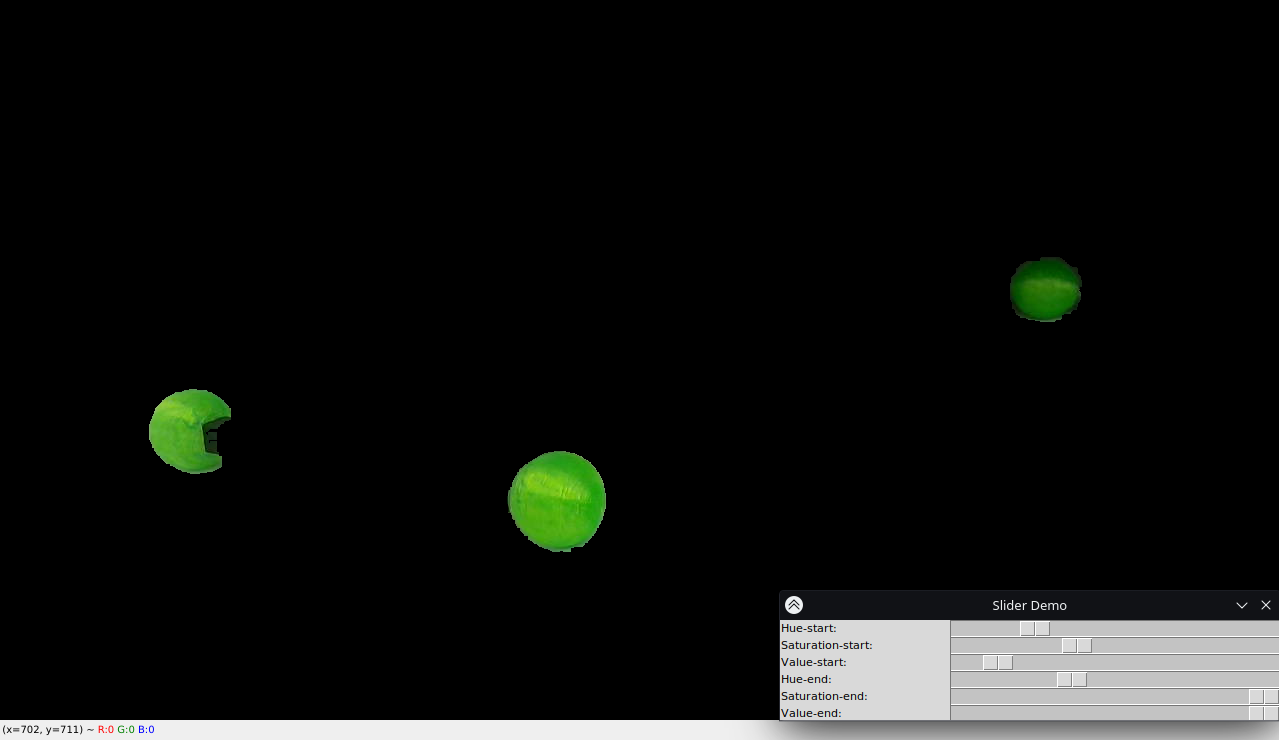
\includegraphics[angle=0,width=\linewidth]{2d-normal-filter.jpg}
    \caption{angewandter Farbfilter}
    \label{Abb: Farbfilter}
  \end{wrapfigure}
  Die Problematik bei dieser Technik liegt in der Unterscheidung des Markers vom Hintergrund. In professionellen, aber sehr viel teuren Systemen, wird auf Infrarot-Kameras und besonders reflektierende kleine Kugeln gesetzt. Dieselbe Technik lässt sich aber auch auf herkömmlichen Webcams anwenden, wenn die Kugeln in einer besonders starken und im Hintergrund nicht vorhandenen Farbe sind. 

  Durch das Konvertieren des aufgenommenen Bildes vom RGB zum HSV-Format (siehe Abbildung \ref{Abb: HSV}), kann man die Daten so filtern, dass nur eine bestimmte Farbe übrigbleibt. Das HSV-Format ist dabei sehr nützlich, da ähnliche Farben (wie beispielsweise hell und dunkelgrün), nah einander liegen, und nur durch Filtern des Farbwertes (Hue), der Farbsättigung (Saturation) und dem Hellwert (Value), eine grobe Maske erstellt werden kann (siehe Abbildung \ref{Abb: Farbfilter}). 
\end{figure}

Beim Testen dieses Konzeptes stellte sich jedoch heraus, dass die Farbe allein nicht genug Kontrast ist, um die Marker zuverlässig vom Hintergrund zu unterscheiden. Bei schlechter oder einseitiger Beleuchtung wurde die Farbe bestimmter Objekte signifikant dunkler, sodass die Filter, die am Tag funktioniert haben, nun gar nicht oder nur unzuverlässig funktionieren würden (siehe Kreise in Abbildung \ref{Abb: Lichtbedingungen}).  

\begin{figure}[htbp!]
  \centering
  \begin{subfigure}[t]{0.45\textwidth}
      \centering
      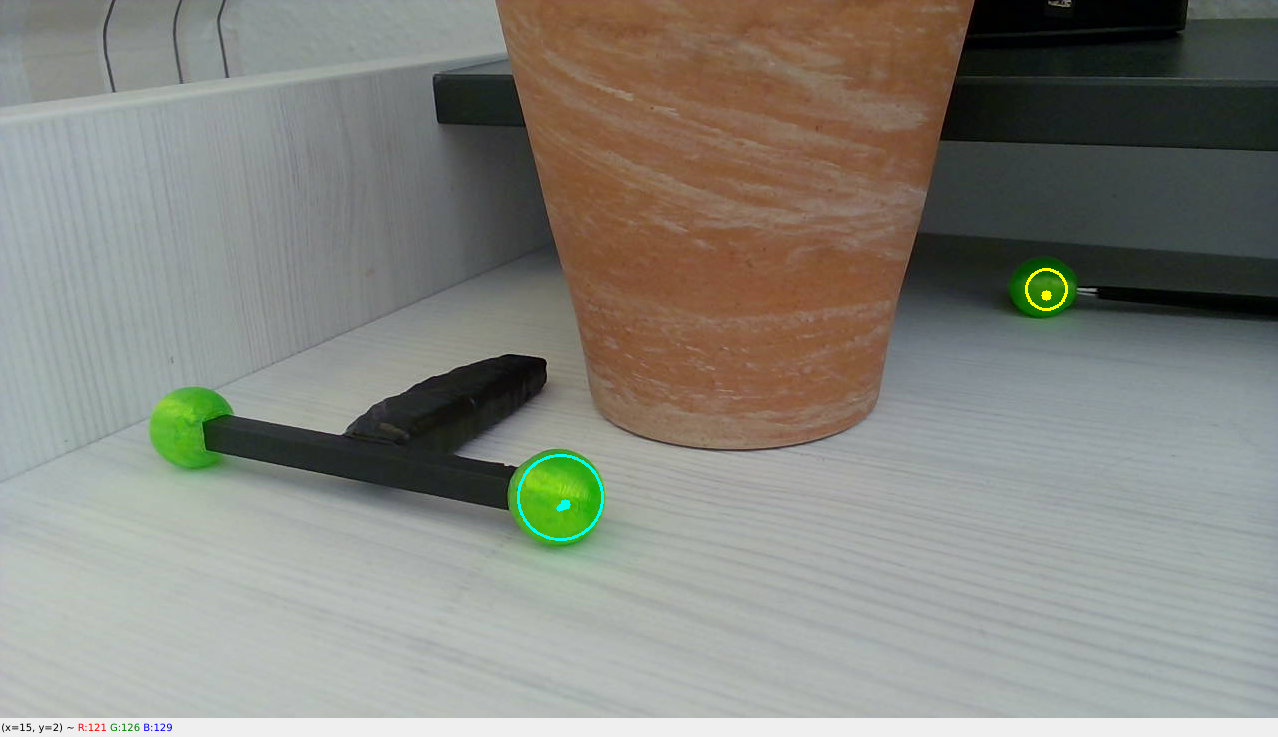
\includegraphics[width=\textwidth]{2d-normal.jpg}
      \caption{normale Lichtverhältnisses}
      \label{Abb: 2d-normal}
  \end{subfigure}
  \hfill
  \begin{subfigure}[t]{0.45\textwidth}
      \centering
      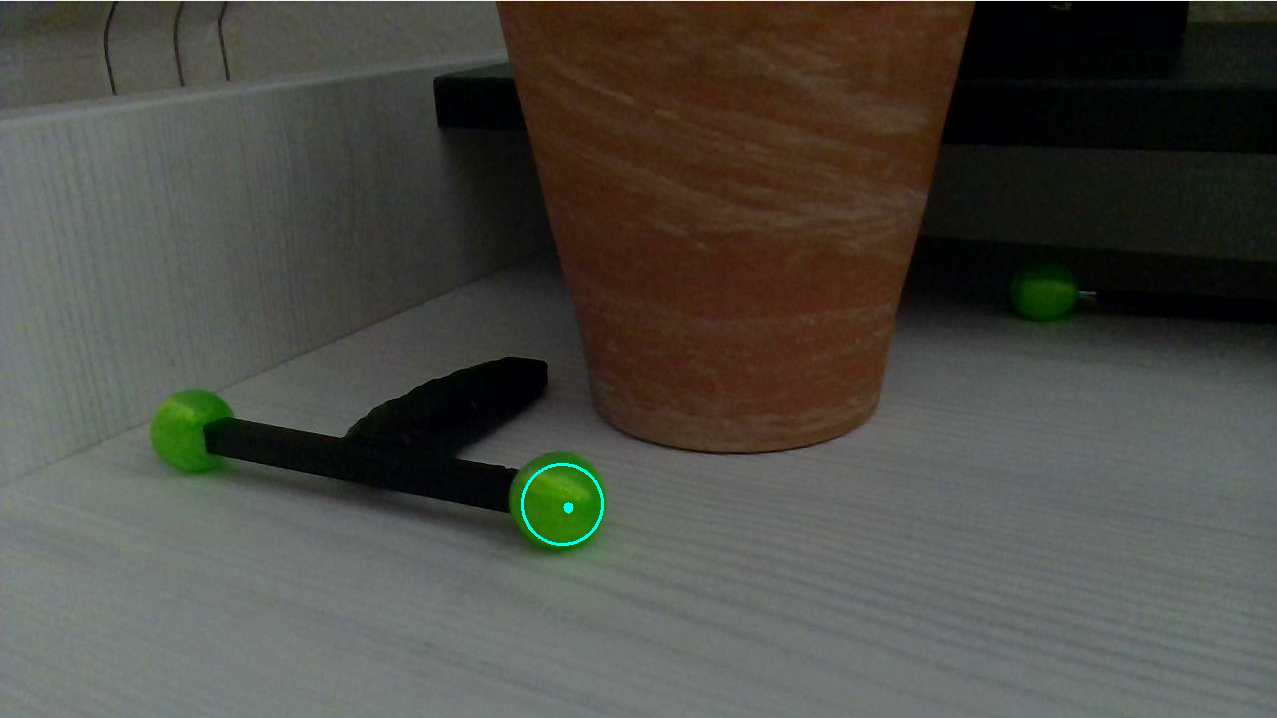
\includegraphics[width=\textwidth]{2d-normal-dark.jpg}
      \caption{dunkle Lichtverhältnisseschrieben}
      \label{Abb: 2d-normal-dunkel}
  \end{subfigure}
  \caption{Tracking Resultate in unterschiedlichen Lichtbedingungen}
  \label{Abb: Lichtbedingungen}
\end{figure}

\begin{wrapfigure}{r}{0.35\textwidth}
  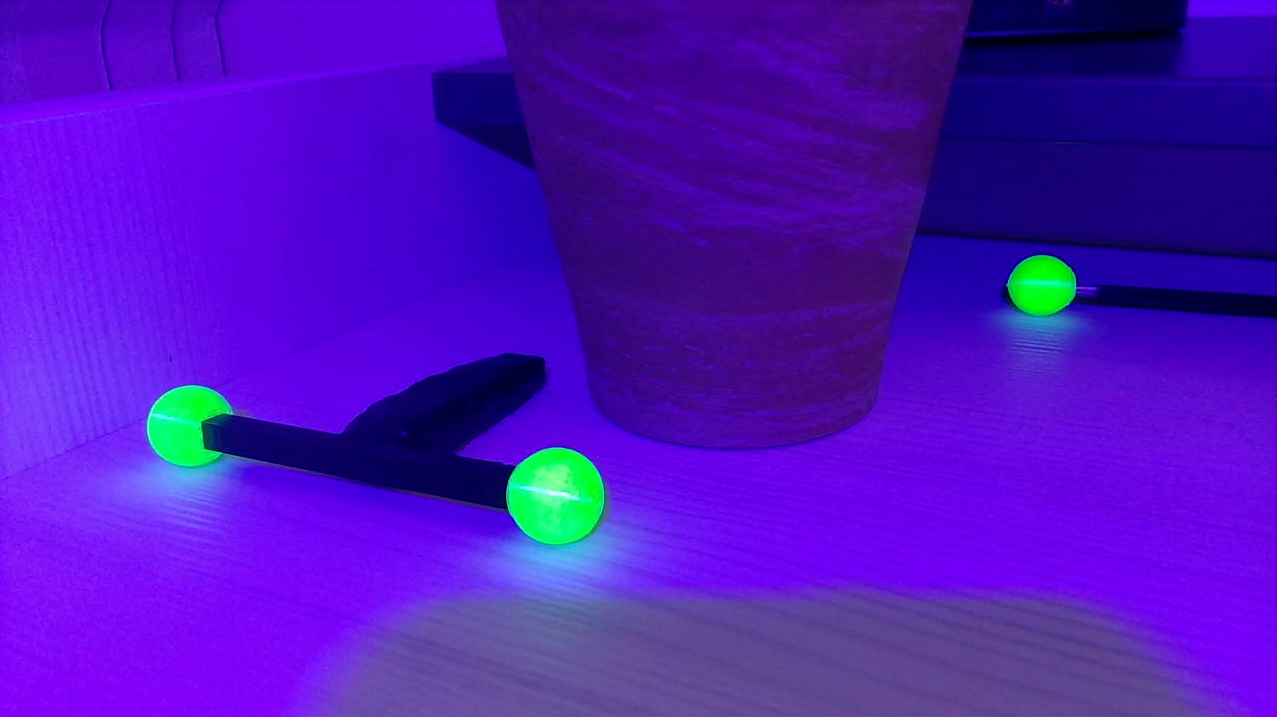
\includegraphics[angle=0,width=\linewidth]{2d-uv-normal.jpg}
  \caption{Farb-Maske nach Bildbearbeitungen}
  \label{Abb: UV}
\end{wrapfigure}
Die ursprüngliche Lösung für dieses Problem ist eine UV-Lampe gewesen, da das grüne Plastik der Kugel das umgangssprachlich genannte „Schwarzlicht“ stark reflektiert, und so stark von anderen Objekten im Raum unterschieden werden konnte. 

Auch wenn diese Lösung in gewissen Fällen funktioniert hat, musste die Stärke der Lampe und die Farbfilter für jede Umgebung neu eingestellt werden, um korrekt zu funktionieren. Ebenfalls war die Qualität des Trackings stark von dem Einfallswinkel des UV-Lichtes abhängig war. Würde dieses nämlich direkt in die Linse der Kamera reflektiert werden, was beim Auftreffen auf eine Kugel immer der Fall ist, würde dieser Bereich möglicherweise komplett weiß werden (siehe Abbildung \ref{Abb: UV}). Anders als Hellgrün ist Weiß eine Farbe, die immer im Hintergrund zu finden ist, und kann daher nicht in die Farbfilter mit integriert werden. 

Eine viel einfachere Lösung ergab sich durch das Experimentieren mit verschiedenen Bildbearbeitungen, die vor dem Tracking Algorithmus auf das Bild angewendet werden.  
Durch das Vermindern des Kontrastes und der Erhöhung der Sättigung sticht die Kugel nun viel stärker aus dem Bild hervor, und kann so deutlich einfacher mit einer Maske ausgeschnitten werden. Zudem verschwindet so der Kontrast zwischen den Seiten der Kugel, wodurch man einen stärker fokussierten Farbfilter verwenden kann, was Messfehler drastisch reduziert.  
Von der übrig gebliebenen Binär-Maske lässt sich relativ einfach das Zentrum einer Kontur und der Radius berechnen, indem eine Kreisform an die Konturen der einzelnen Masken angenähert wird, bis diese den Rand der Kontur erreicht. Durch diese Technik kann das Zentrum einer Kugel selbst dann
\begin{figure}[htbp!]
  \centering
  \begin{subfigure}[t]{0.45\textwidth}
      \centering
      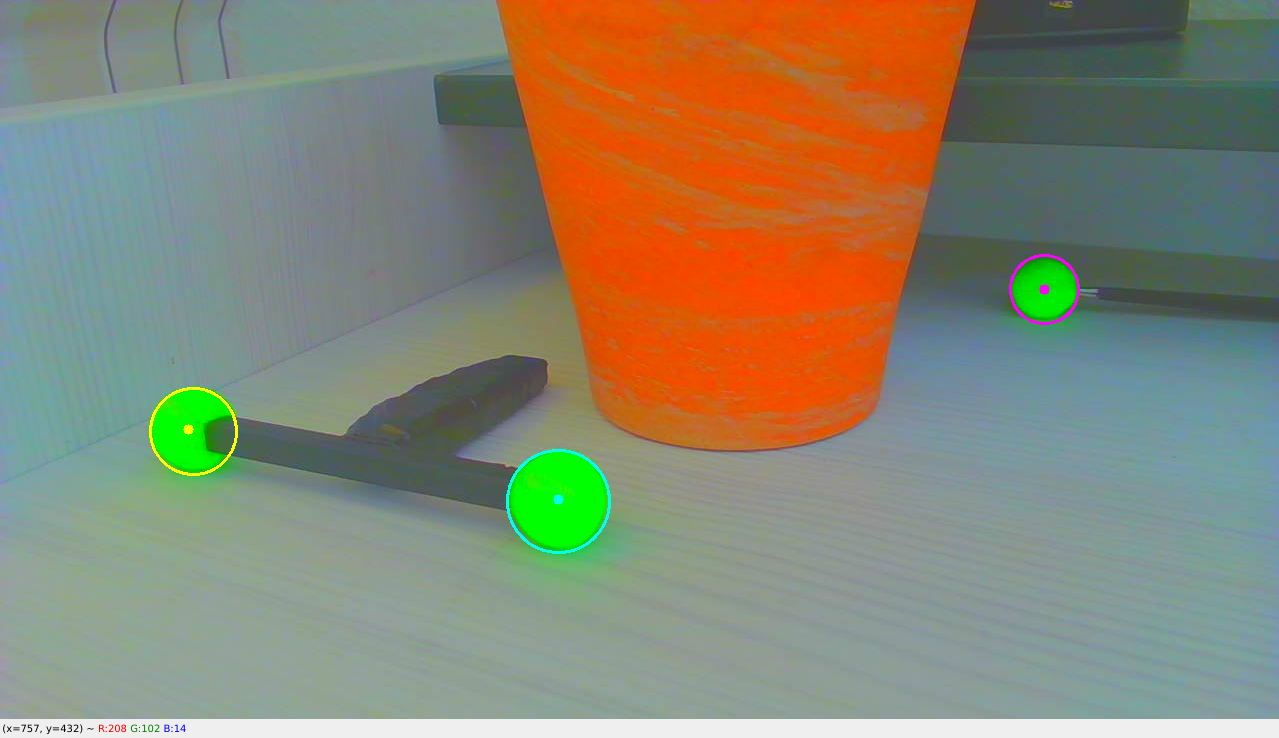
\includegraphics[width=\textwidth]{2d-color.jpg}
      \caption{normale Lichtverhältnisses}
      \label{Abb: 2d-color-normal}
  \end{subfigure}
  \hfill
  \begin{subfigure}[t]{0.45\textwidth}
      \centering
      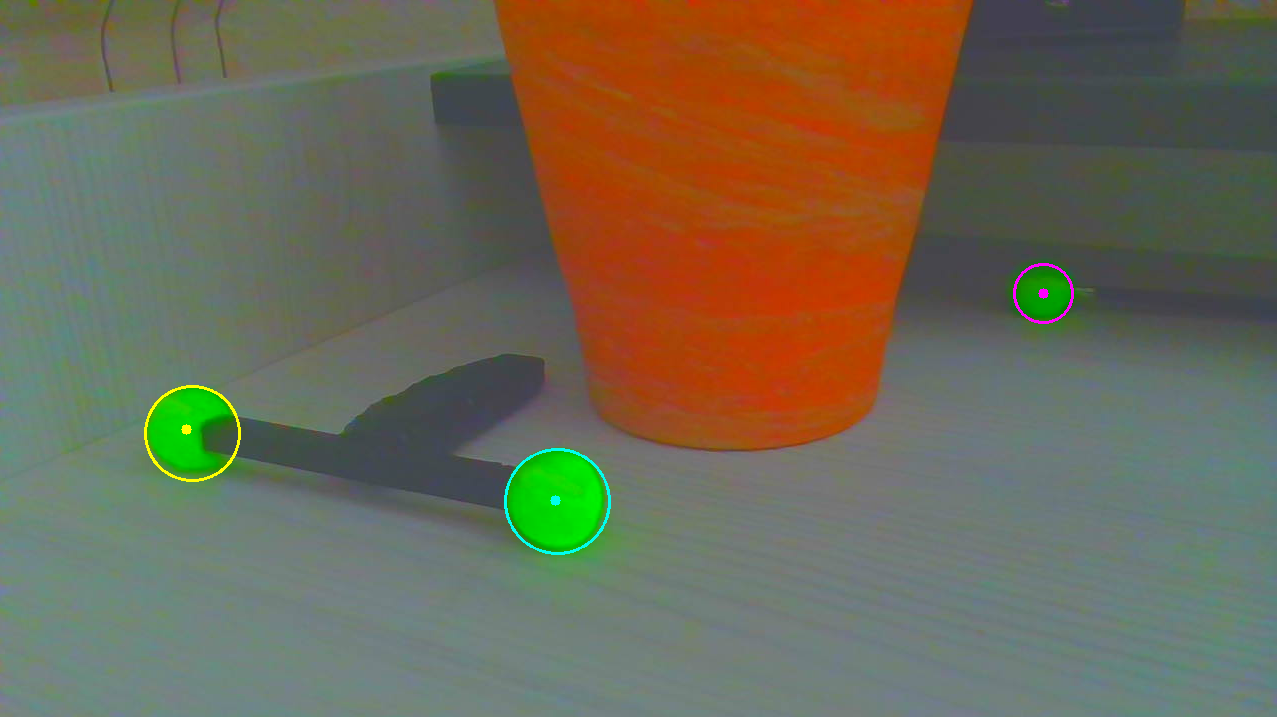
\includegraphics[width=\textwidth]{2d-color-dark.jpg}
      \caption{dunkle Lichtverhältnisseschrieben}
      \label{Abb: 2d-color-dunkel}
  \end{subfigure}
  \hfill
  \vspace{10pt}
  \begin{subfigure}[t]{0.6\textwidth}
      \centering
      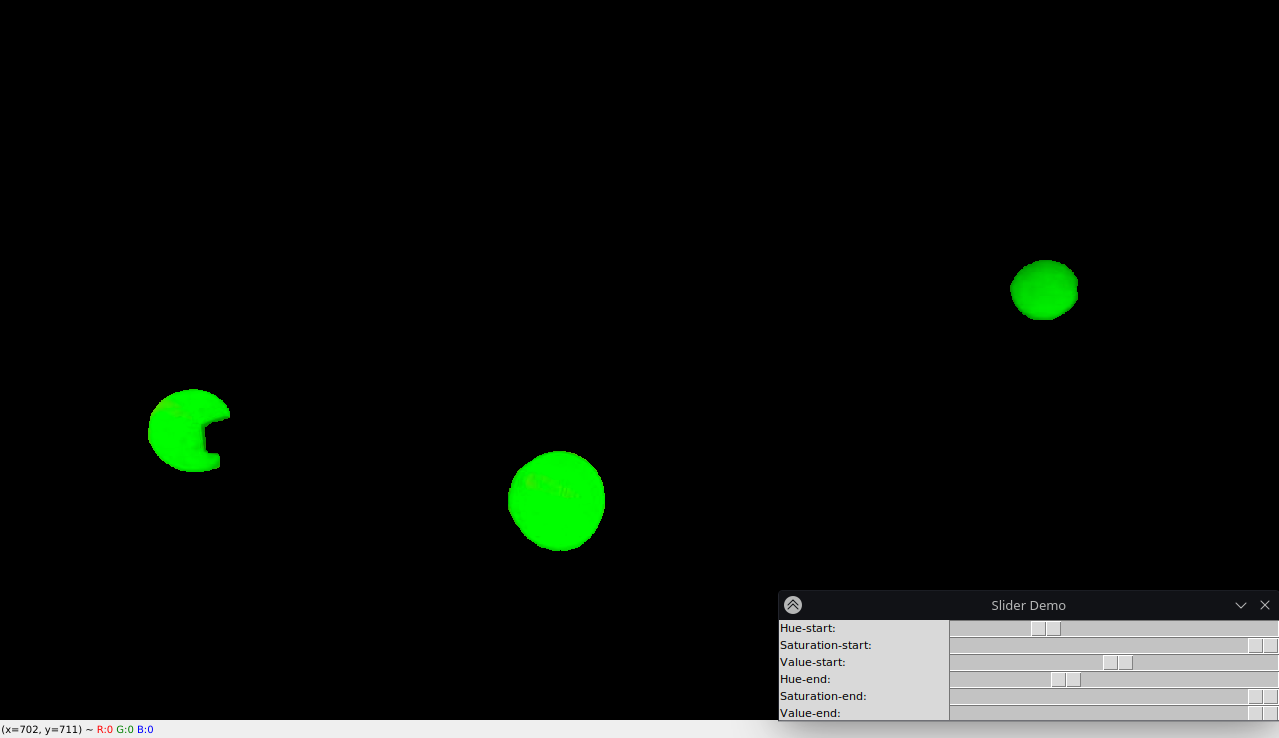
\includegraphics[width=\textwidth]{2d-color-filter.jpg}
      \caption{resultierende Maske}
      \label{Abb: 2d-color-maske}
  \end{subfigure}
  \caption{Tracking Resultate in unterschiedlichen Lichtbedingungen mit Nachbearbeitung}
  \label{Abb: Nachbearbeitungen}
\end{figure}

\subsubsection{Identifizierung der Objekt}
Auch wenn es für die meisten Anwendungen nicht nötig ist, können verschiedene Tracking Punkte durch zwei unterschiedliche Methoden im zeitlichen Verlauf und selbst in Bewegung voneinander unterschieden werden. Einerseits können mehrere Tracking-Farben hinzugefügt werden, zum Beispiel eine rote, blaue und grüne Kugel, andererseits vergibt der Tracking-Algorithmus jeder Kontur eine ID, und versucht im nächsten Frame diese anhand der Nähe zu den neuen Ergebnissen zum selben zuzuteilen. In der Praxis funktioniert die zweite Technik trotz ihrer Simplizität erstaunlich gut, sogar beim Überkreuzen zweier Laufbahnen.  

\subsection{Kamera-Kalibrierung}
Um die aus dem 2D-Tracking gewonnenen Daten in den dreidimensionalen Raum zu übertragen, benötigt man diverse Informationen, die sich in intrinsische und externe Parameter gruppieren lassen. Ersteres sind dabei die Eigenschaften der Kamera selbst, also Brennweite, Verzerrung und Auflösung, welche den geometrischen Zusammenhang zwischen dem Welt- und Bildkoordinatensystem. Aus ihnen lässt sich die Projektion eines 2D-Bildpunktes in den 3D-Raum errechnen. 

Da außer der Auflösung keine Parameter bekannt sind, müssen diese durch eine Kamera-Kalibrierung geschätzt und in folgende Berechnungen mit integriert werden. Die perspektivische Transformation eines Bildpunktes lässt sich mathematisch so beschreiben:
\begin{figure}[hbtp!]
    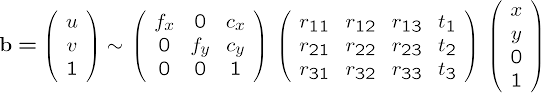
\includegraphics[width=\textwidth]{camera_matrix.png}
    \caption{Berechnung der homogenen Koordinaten im dreidimensionalen Raum}
    \label{Abb: camera_matrix}
\end{figure}

Um aus den 2D-Bildkoordinaten $u$ und $v$ den projizierten Punkt im dreidimensionalen Raum zu erhalten, muss der homogene Vektor mit der Kamera Matrix multipliziert werden. Diese besteht aus der horizontalen und vertikalen Brennweite $fx$ und $fy$, und den Koordinaten des Bildzentrums $cx$ und $cy$ (siehe Abbildung \ref{Abb: camera_matrix}).

\begin{wrapfigure}{R}{0.35\textwidth}
  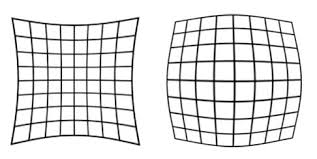
\includegraphics[width=\linewidth]{distortion.jpeg}
  \caption{zwei Formen von Verzerrung}
  \label{Abb: distortion}
\end{wrapfigure}
Des Weiteren muss die durch Kamera-Linsen entstehende Verzerrung rückgängig gemacht werden, wofür 5 Parameter gebraucht werden, die die Stärke, Form und Richtung der Verzerrung beschreiben (siehe Abbildung \ref{Abb: distortion}).

Da diese Parameter für jede Kamera unterschiedlich sind und bei herkömmlichen Webcams nicht vorgegeben sind, müssen sie durch eine Kamera-Kalibrierung geschätzt werden. Hierfür bietet sich die ROS-Library "camera\_calibration" an, da sie die gewonnenen Daten direkt in einem für ROS verständlichen Format abspeichert und diese dann von dem Modul "camera\_info" im System freigegeben (published) werden können.

Die nötigen intrinsischen Parameter werden berechnet, indem man mehrere Bilder eines Schachbrettes mit bekannten Abmessungen macht, und anhand der Positionierung und Verformung von Linien und Punkten die nötigen Parameter berechnet. Es ist dabei wichtig, diesen Prozess für jede Kamera zu wiederholen, da selbst bei identischem Hersteller und Modell die Werte unterschiedlich seien können.

\vspace{10pt}
\begin{figure}[htbp!]
  \centering
  \begin{subfigure}[c]{0.45\textwidth}
    \centering
    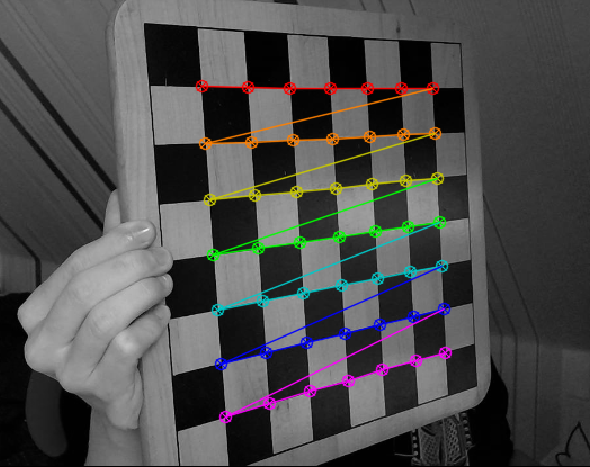
\includegraphics[width=\textwidth]{calibration.png}
    \caption{Kalibrierungsprozess mithilfe eines Schachbrettes}
    \label{Abb: calibration}
  \end{subfigure}
  \hfill
  \begin{subfigure}[c]{0.45\textwidth}
      \centering
      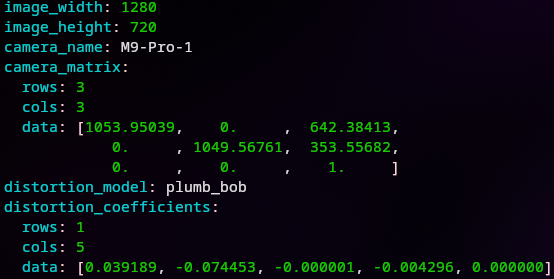
\includegraphics[width=\textwidth]{calibration-data.png}
      \caption{resultierende Parameter}
      \label{Abb: calibration-data}
  \end{subfigure}
  \caption{Prozess und Ergebnisse einer Kamerakalibrierung}
  \label{Abb: camera_calibration}
\end{figure}

\subsubsection{System-Integration der Kamerakalibrierung}
Um das System besonders leicht bedienbar zu machen, übernimmt das Modul "camera\_info" viele Aufgaben, die sonst manuell erledigt werden müssen. Beim Starten des Systems durch den "Manager" (siehe Abschnitt Systemaufbau) wird für jede angeschlossene Kamera ein solches Modul gestartet, welches dann auf Basis des Gerätenamen des vom Manager zugewiesenen USB-Ports das Modell erkennt und nach abgespeicherten Konfigurationen sucht. Wenn eine solche gefunden wurde, wird die Kamera-Matrix, die Verzerrungs-Parameter und die Auflösung auf dem "camX/camera\_info" Topic freigegeben, sodass sowohl Visualisierungssoftware als auch andere Module auf die Kamera spezifischen Parameter zugreifen können. Wenn keine bekannte Konfigurationen gefunden wurde, wird der Nutzer benachrichtigt und zum Kalibrierungsprozess weitergeleitet.

\subsection{Positions-Kalibrierung}
Um die unterschiedlichen Kamera-Perspektiven im dreidimensionalen Raum in Relation zu setzen, werden die extrinsischen Parameter benötigt. Diese beschreiben die Pose der Kamera, also die Translation und Rotation im Raum. Da diese Werte für jedes aufgebaute 3D-Tracking-System unterschiedlich sind und den größten Einfluss auf die Präzision und Richtigkeit der berechneten Position eines Objektes haben, wird eine Positions-Kalibrierung benötigt, die es dem Nutzer ermöglicht, die Pose der einzelnen Kameras anhand von Daten akurat schätzen zu lassen. 

\subsubsection{Theorie}
Die Pose einer Kamera im Weltkoordinatensystem lässt sich mit der sogenannten essenziellen Matrix beschreiben, unter der Bedingung, dass die intrinsischen Parameter der Kamera bekannt sind. Diese Matrix besteht aus der Rotations-Matrix und dem Translations-Vektor und beschreibt daher die 6 Freiheitsgrade. Folglich lässt sich Abbildung \ref{Abb: camera_matrix} so erweitern:

\begin{figure}[hbtp!]
    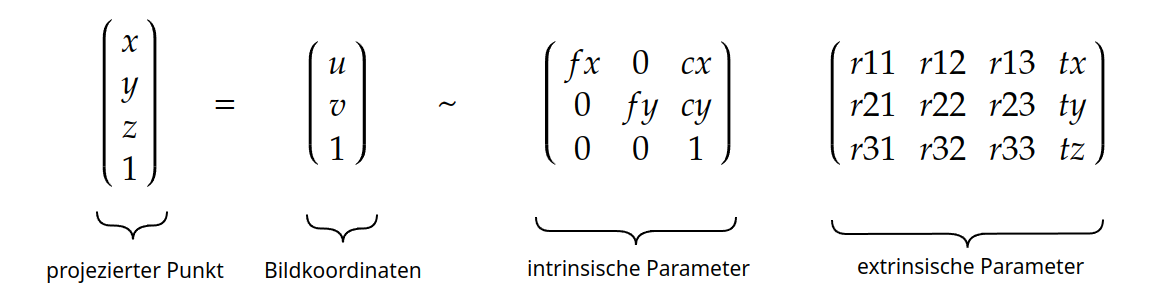
\includegraphics[width=\textwidth]{matrix_shit.png}
    \caption{Berechnung der homogenen Koordinaten im dreidimensionalen Raum mit extrensischen Parametern}
    \label{Abb: essential_matrix}
\end{figure}

Zur Schätzung dieser Matrix wird im Bereich der "computer vision" meist der Prozess "visuelle Odometrie" verwendet, welcher die Berechnung der relativen Pose zweier visuellen Perspektiven durch Analysieren von Kamerabildern beschreibt. Möglich ist dies, da die projizierten Bildpunkte in perspektivischer Relation zueinander Informationen über die relative Position der Kameras untereinander enthalten, und diese durch bestimmte Algorithmen geschätzt werden können.

Ein solches Verfahren lässt sich in folgende Schritte einteilen:

\begin{enumerate}
  \item Beide Perspektiven werden mit einem Algorithmus auf gut zu identifizierende Punkte untersucht, meiste kontrastreiche Ecken und Kanten.
  \item Die gefundenen Punkte werden anhand ihrer Umgebung und visuellen Eigenschaften zueinander zugeteilt. Dies ist nur möglich, wenn beide Kameras dieselbe Szene beobachten.
  \item Zwischen den nun gefundenen ``Punktepaaren'' lassen sich
  Epipolarlinien ziehen (siehe Abbildung \ref{Abb: epipolar}), welche es, mit der Projektionsmatrix der Kamera (siehe
  Kamera-Kalibrierung) zusammen, einem sogenannten N-Punkt-Algorithmus
  ermöglichen, eine zugehörige essenzielle Matrix anzunähern.
  \item Das Verfahren wird mehrmals auf unterschiedlich ausgewählte Gruppen
  von Punkten angewendet, und die geschätzten Positionen mithilfe des RANSAC
  Algorithmus von Ausreißern gefiltert.
\end{enumerate}

\begin{figure}[hbtp!]
    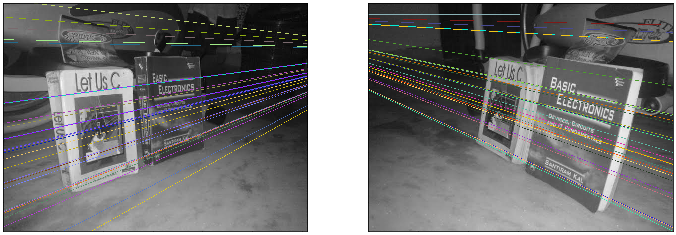
\includegraphics[width=\textwidth]{epipolar_2.png}
    \caption{Epipolarlinien zweier Perspektiven}
    \label{Abb: epipolar}
\end{figure}

Die genaue Funktionsweise aller genannter Algorithmen werden in folgenden Quellen beschrieben: 

\subsubsection{Anpassung des Verfahrens}
Da das oben beschriebene Verfahren überwiegend für das Bestimmen einer Kamerabewegung verwendet wird, also die unterschiedlichen Perspektiven von derselben Kamera zeitlich versetzt aufgenommen werden, gäbe es in dieser Anwendung bestimmte Faktoren, die die Leistung des Verfahrens beeinträchtigen würden.
Einerseits ist die Qualität der Schätzung stets von der Menge an gefundenen Epipolarlinien abhängig, welche wiederum von einem kontrastreichen Hintergrund mit vielen Konturen abhängig sind. Andererseits ist die Positionierung der Kameras eingeschränkt, da diese stets identische Konturen im Bild haben müssen.

Um dieses Problem zu umgehen, verwendet das System einen umgekehrten "Structure from Motion" Ansatz, indem durch das Bewegen eines Objektes in den Perspektiven der Kameras unendliche viel Punktpaare erstellt werden können. 

Es gibt mehrere N-Punkt-Algorithmen, unter anderem den 5-, 7- und 8-Punkt-Algorithmus. In einem Vergleich dieser drei (siehe ...), hat sich der 5-Punkt-Algorithmus als weitaus zuverlässiger herausgestellt, da er im Vergleich zu den Alternativen nur 5 Freiheitsgrade besitzt. In der Translation geht nämlich die Skalierung verloren, weshalb nur ein Einheitsvektor übrig bleibt. Trotz dieses Nachteils wird die OpenCV Implementation des Algorithmus in Verbindung mit RANSAC genutzt, um die Pose zu schätzen.

\newpage
Der Prozess lässt sich nun also wie folgt darstellen:

\begin{enumerate}
  \item Ein Stab mit einem grünen Ball am Ende wird im Bild aller Kameras bewegt.
  \vspace{10pt}
  \begin{figure}[hbtp!]
      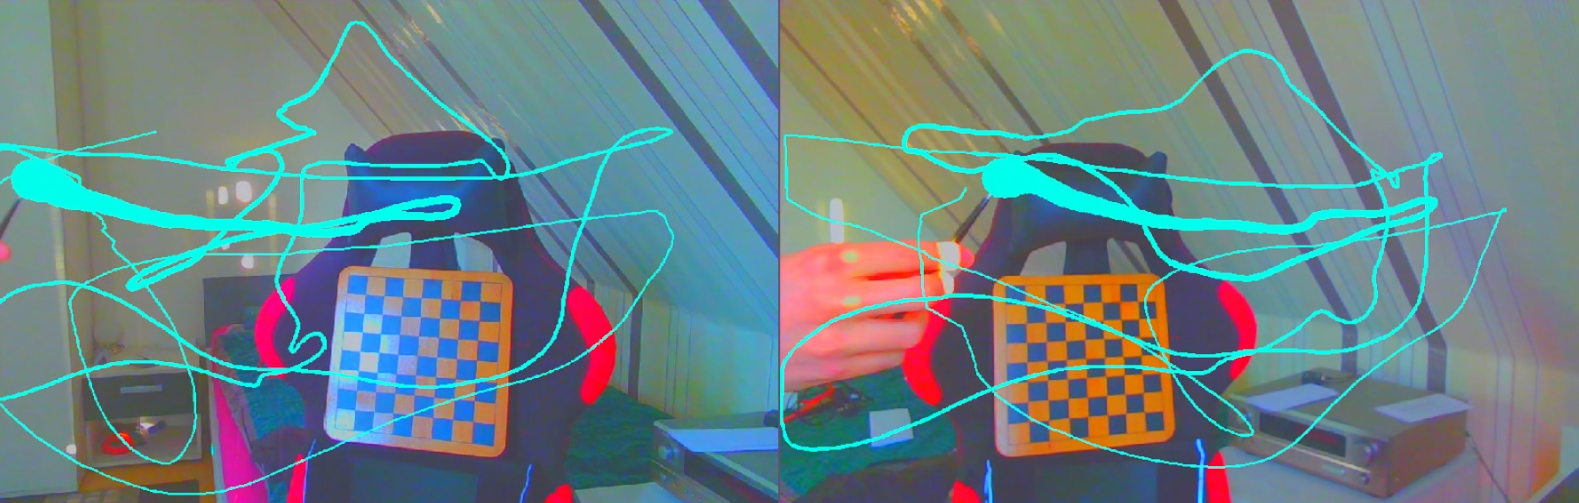
\includegraphics[width=\textwidth]{crack.png}
      \caption{Aufgenommene Positionen des Objektes im zeitlichen Verlauf}
      \label{Abb: wand}
  \end{figure}
  
  \item Während dieses Prozesses wird nach jedem aufgenommenen Bild überprüft, ob das Punktepaar fehlerfrei ist. Hierfür muss die Aufnahmezeitpunkte weniger als 0.01s zeitliche Differenz besitzen, und in jedem Frame exakt 1 Objekt erkannt worden sein.
  \item Das Punktepaar wird nun einer Liste hinzugefügt, die ein 5-Punkt-Algorithmus verwendet, um eine essenzielle Matrix zu schätzen. 
  \item Eine kontinuierlich laufender RANSAC-Schleife überprüft die geschätzten Posen auf Ausreißer und filtert dies aus der Liste an Posen.
  \item Nach einer bestimmten Anzahl an Durchläufen (zwischen 1000 und 4000), welche abhängig von den Fehlern der aufgenommenen Daten ist, wird der Durchschnitt der finalen Translationen und Rotationen berechnet, um kleinere Verwacklungen zu filtern.
\end{enumerate}

\subsubsection{System-Integration und Entwicklung der Positions-Kalibrierung}
Auch wenn es bereits einige Libraries für die Implementierung des 5-Punkt-Algorithmus gab, sind diese in anderen Szenarien verwendet worden, weshalb ich in der Entwicklung auf kein funktionierendes Beispiel zurückgreifen konnte. Des Weiteren sind Algorithmen der visuellen Odometrie meist sehr sensibel und müssen daher mit vielen Parametern abgestimmt und gefiltert werden, was auch ein weiteres Problem in der Entwicklung darstellt: Der Fortschritt ist meist nicht linear. Die Anzahl an Werten und Einflüssen, die die Resultate dramatisch beeinflussen können, ist sehr groß, was die Problemsuche sehr mühselig gestaltet. Ein Beispiel ist die Brennweite der Kamera; wenn dieser durch die Kamera-Kalibrierung geschätzter Wert mehr als 10\% von dem realen Wert entfernt ist, nähert sich der 5-Punkt-Algorithmus keinem finalen Wert mehr an. 

Um die Entwicklung der Positions-Kalibrierung zu erleichtern, mussten einige Fehlerquellen durch das Nutzen synthetischer Daten vorerst vernachlässigt werden, ohne sich zu weit von reellen Bedingungen zu entfernen. 

Hierfür wurde in der Entwicklung auf die Simulationsumgebung "Gazebo" gesetzt, da sie sich ideal in ROS integrieren lässt. Hier simulierte man unterschiedliche Kamera-Positionen im Raum mit verschiedener "Schwierigkeit", und ließ einen simulierten grünen Ball eine Strecke im Raum "abfahren". Gazebo simulierte nun das Sichtfeld der Kameras, die Auflösung und die intrinsischen Parameter und veröffentlichte die Daten im ROS Netzwerk. Praktisch wird so das "camera\_driver" und "camera\_info" Modul ersetzt, ohne die Funktionalität des Systems zu beeinflussen (siehe Abbildung \ref{Abb: calibration-aufbau}). 
Wenn der Nutzer das Kalibrierungs-Modul startet, subscribed dieses zu allen Topics, die Informationen für den Prozess veröffentlichen und sendet die geschätzten Posen an das "camera\_position" Modul.

\begin{figure}[hbtp!]
    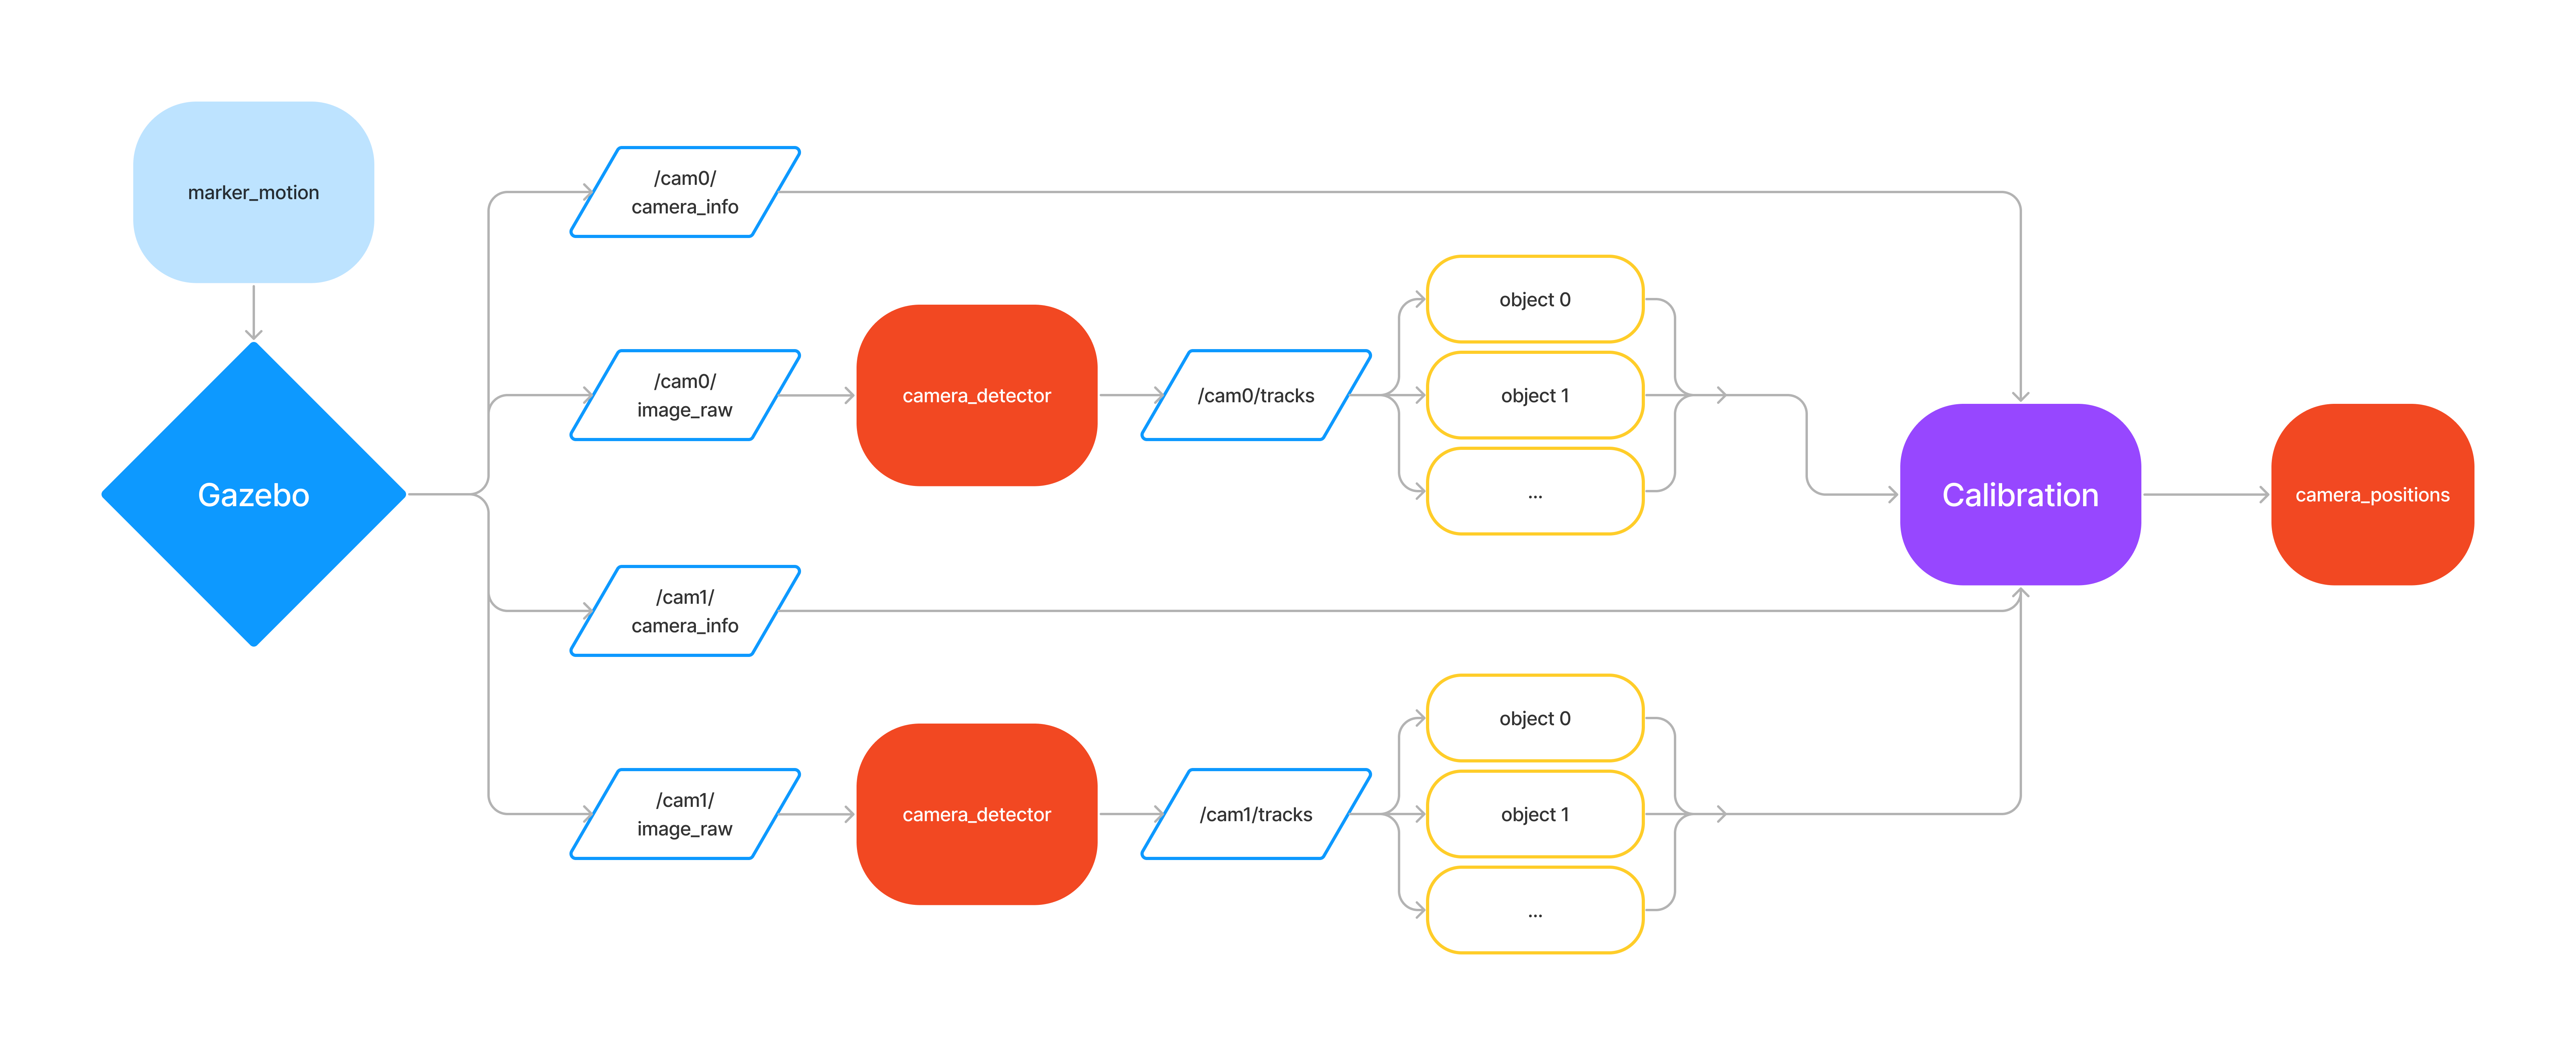
\includegraphics[width=\textwidth]{anytrack-calibration.png}
    \caption{Systemaufbau mit der Integration einer Simulationssoftware}
    \label{Abb: calibration-aufbau}
\end{figure}
Ein laufender Kalibrierungsprozess sieht dann etwa so aus:
\vspace{5pt}
\begin{figure}[hbtp!]
    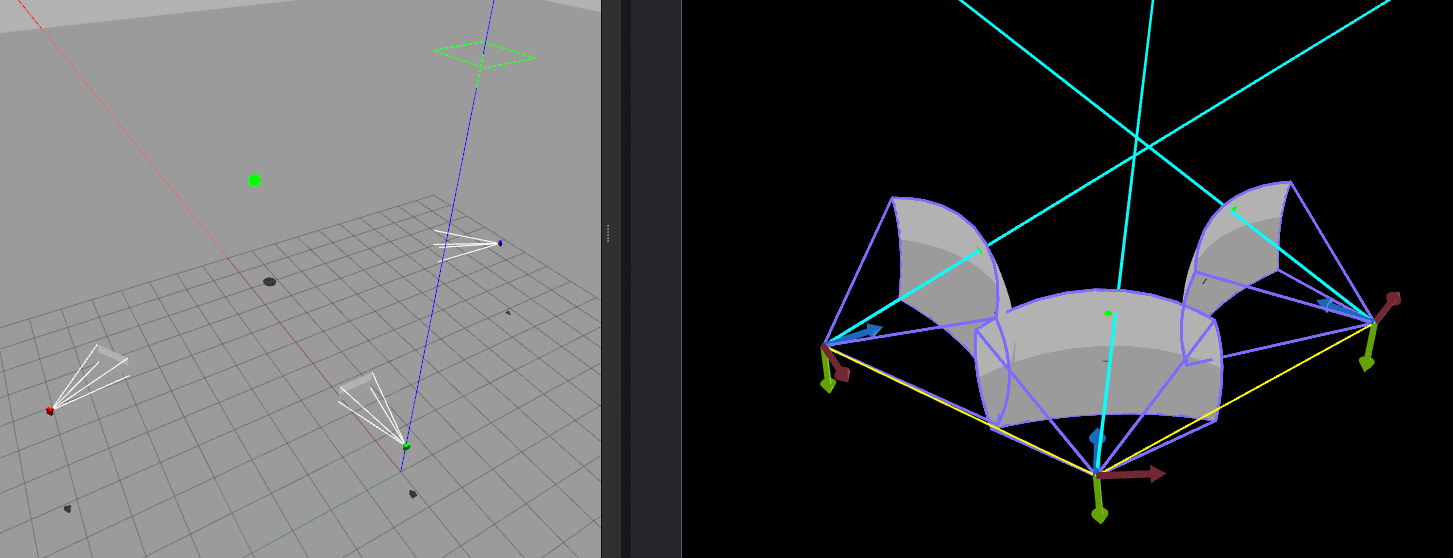
\includegraphics[width=\textwidth]{simulation_calibration-2.png}
    \caption{Links: Gazebo Simulation, Rechts: Visualisierung der geschätzten Kamera Posen}
    \label{Abb: simulation-calibration}
\end{figure}

\subsubsection{Anwendung auf reelle Daten}
Auch wenn der Prozess an synthetischen Daten kontinuierlich verbessert wurde und die Pose präzise genug bestimmt werden kann, gibt es einige Probleme, die behoben werden müssen, um die Kalibrierung auch in reellen Bedingungen durchführen zu können. 

Zunächst funktioniert der 5-Punkt-Algorithmus nur, wenn alle Punkte aus Kameras mit identischer Kamera-Matrix kommen, was selbst bei identischen Modellen nie der Fall ist. Die durch das Kontur-Tracking gefundenen Objekte müssen daher in ein kanonisch kameraübergreifendes Bildkoordinatensystem versetzt werden, hierfür werden die Bildkoordinaten eines Objektes, zum Beispiel (834px, 789px), auf Basis der intrinsischen Parameter und der Auflösung von einem 1280x720px auf ein 1x1px System projiziert. Die Bildpunkte werden so "entzerrt" und können vom 5-Punkt-Algorithmus verwendet werden.

Des Weiteren leidet die Präzision der Schätzung von der größeren Anzahl an visuellen Fehlern, wie zum Beispiel unterschiedliche Lichtverhältnisse, zu schnelle Bewegungen oder abweichende Kamera-Parameter. Um dies zu umgehen, muss die Filterung der Ausreißer in der Kameraschätzung optimiert werden, wofür der RANSAC-Algorithmus zuständig ist. Ein Beispiel dafür ist die Schätzung der Translation, welche aufgrund der nicht vorhandenen Skalierung stets auf einer Sphäre um (0,0) mit dem Radius 1 liegt. 

\vspace{5pt}
\begin{figure}[hbtp!]
    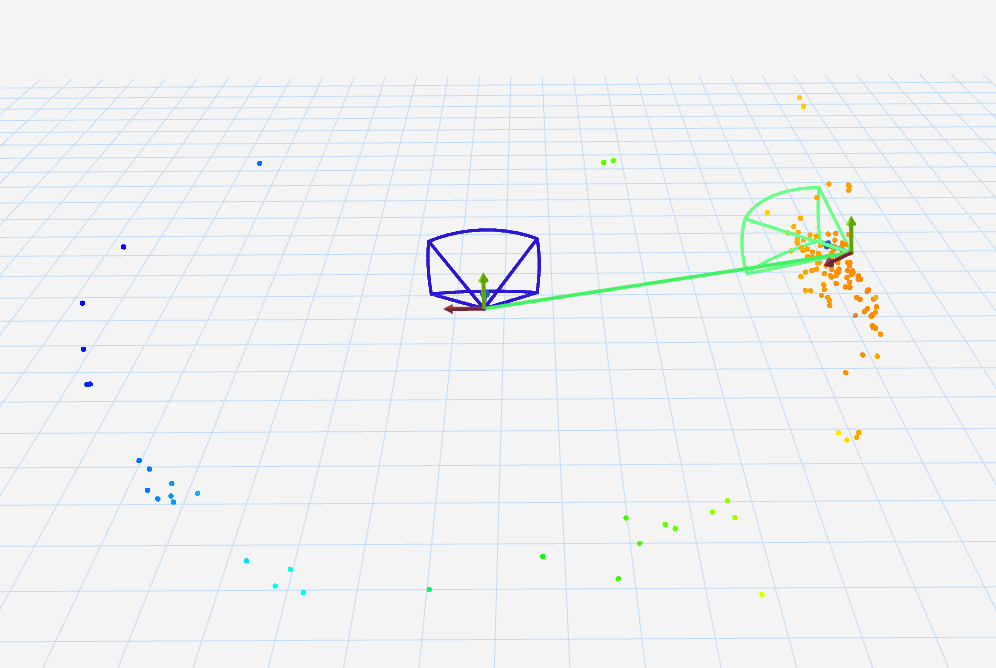
\includegraphics[width=\textwidth]{pointcloud_no_filter.png}
    \caption{Geschätzte Transformation-Werte im zeitlichen Verlauf, während der Aufnahme einer Kalibrierungssequenz auf Basis reeller Daten. Die grüne Kameraperspektive zeigt den finalen Schätzwert nach 200 aufgenommen Werten.}
    \label{Abb: pointcloud_no_filter}
\end{figure}


\begin{figure}[hbtp!]
    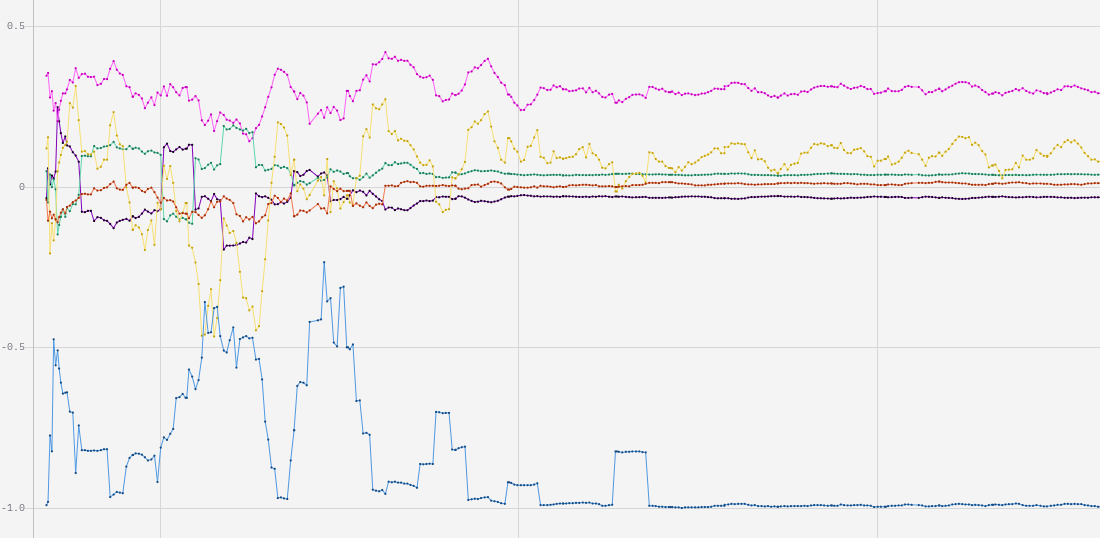
\includegraphics[width=\textwidth]{calibration_graph_white.png}
    \caption{Geschätzte Transformations- und Rotations-Werte im zeitlichen Verlauf, graphisch dargestellt}
    \label{Abb: calibration_graph}
\end{figure}

\vspace{10pt}

\begin{figure}[hbtp!]
    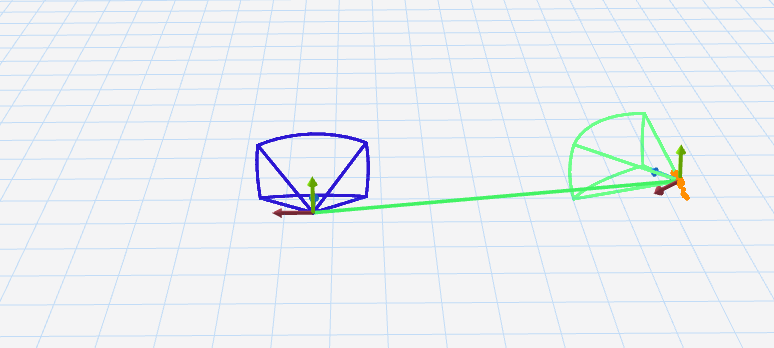
\includegraphics[width=\textwidth]{pointcloud_with_filter.png}
    \caption{Abbildung \ref{Abb: pointcloud_no_filter} ohne die ersten 100 geschätzten Werte und mit angepasster Filterung}
    \label{Abb: pointcloud_with_filter}
\end{figure}

\vspace{10pt}

\subsubsection{Schätzung der Skalierung}
Da bei der Schätzung der essenziellen Matrix die Skalierung, also die Länge des
Translations-Vektors, verloren geht, kann beim Verwenden zweier Kameras die
Position eines Objektes nur noch relativ bestimmt und keine genauen Maße durch
das 3D-Tracking-System errechnet werden. Bei der Verwendung von mehr als zwei
Perspektiven ist die Schätzung des Objektstandortes ohne die Skalierung nicht
mehr möglich, da die Vektoren sich nun nicht mehr am selbem Ort schneiden.
Folglich muss die Skalierung durch eine weitere Kalibrierung erfasst werden,
wofür ein Objekt mit bekannten Abmessungen nötig ist. Ähnlich wie bei der
Schätzung der intrinsischen Parameter, bietet sich auch hier ein Schachbrett an,
da es durch die vielen kontrastreichen Ecken und Kanten leicht zu tracken ist.

In einem Bild lässt sich nun, nach der Entzerrung mit den intrinsischen
Parametern der Kamera, die Neigung des Brettes errechnen und bei zusätzlichem in
Betracht ziehen der Projektions-Matrix und Abmessungen der einzelnen
Schachfelder, die Entfernung vom Objekt zur Kamera schätzen.

Dieser Abstand wird mit dem geschätzten Abstand durch das 3D-Tracking-System
verglichen und die Skalierung der einzelnen Translationen so weit angepasst, bis
diese identisch mit dem Vergleichswert sind. Der Prozess wird zum Vermindern von
Messfehlern mehrmals wiederholt und der Durchschnitt der Werte gespeichert.

\subsection{3D-Vektoren}

\section{Ergebnisse}

%%%%%%%%%% Quellenverzeichnis
\newpage
\nocite{*}
\bibliography{refs}{}
\bibliographystyle{plain} 
\end{document}